\documentclass[11pt,fleqn]{article}

\usepackage{../../mainStructure}

% Proposition box. Just for these notes
\newmdenv[skipabove=7pt,
skipbelow=7pt,
rightline=true,
leftline=true,
topline=true,
bottomline=true,
linecolor=darkgunmetal,
innerleftmargin=5pt,
innerrightmargin=5pt,
innertopmargin=5pt,
leftmargin=0cm,
rightmargin=0cm,
linewidth=1pt,
backgroundcolor=eggblue!5,
innerbottommargin=5pt]{pBox}	
\renewenvironment{prop}{\begin{pBox}\begin{propT}}{\end{propT}\end{pBox}} 

%%\ifoptionfinal{
%\usepackage[
%	active,
%	generate=SFP_Props,
%	extract-cmd= section,
%	extract-env={prop}
%]{extract}
%\begin{extract}
%\usepackage{../../../mainStructure}
%\fancyhf{}
%\fancyhead[L]{Symmetries Fields and Particles}
%\fancyhead[R]{Propositions}
%\end{extract}
%%}{\relax}

\begin{document}

%\begin{extract*}
\title{Symmetries, Fields and Particles\\
\Large{Summary Notes} \\ \hrulefill}
\author{Sam Crawford\\
\large{\textsl{Based on the Course Given by Nick Dorey}}}
\date{Michaelmas 2017}

\maketitle
%\end{extract*}
\begin{center}
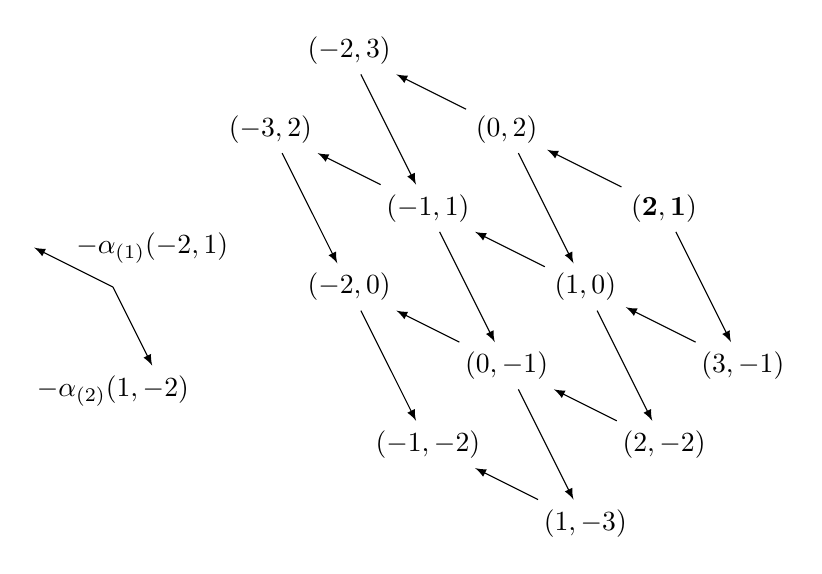
\begin{tikzpicture}


\draw [-latex] (-5,0) -- (-4.5,-1);
\draw [-latex] (-5,0) -- (-6,0.5);
\node [below] at (-5,-1) {$ -\alpha_{(2)} \rightsquigarrow (1,-2)$};
\node at (-4.5,0.5) {$-\alpha_{(1)} \rightsquigarrow (-2,1)$};



\node (v12) at (2,1) {$\mathbf{(2,1)}$};
\node (v13) at (3,-1) {$(3,-1)$};
\draw [-latex] (v12) edge (v13);
\node (v15) at (0,2) {$(0,2)$};
\node (v16) at (-2,3) {$(-2,3)$};
\draw [-latex] (v12) edge (v15);
\draw [-latex] (v15) edge (v16);
\node (v14) at (1,0) {$(1,0)$};
\node (v17) at (2,-2) {$(2,-2)$};
\draw [-latex] (v15) edge (v14);
\draw [-latex] (v14) edge (v17);
\node (v18) at (-1,1) {$(-1,1)$};
\node (v19) at (0,-1) {$(0,-1)$};
\node (v20) at (1,-3) {$(1,-3)$};
\draw [-latex] (v16) edge (v18);
\draw [-latex] (v18) edge (v19);
\draw [-latex] (v19) edge (v20);
\node (v21) at (-1,-2) {$(-1,-2)$};
\draw [-latex] (v20) edge (v21);
\draw [-latex] (v17) edge (v19);
\draw [-latex] (v14) edge (v18);
\node (v22) at (-2,0) {$(-2,0)$};
\draw [-latex] (v19) edge (v22);
\draw [-latex] (v13) edge (v14);
\node (v23) at (-3,2) {$(-3,2)$};
\draw [-latex] (v18) edge (v23);
\draw [-latex] (v23) edge (v22);
\draw [-latex] (v22) edge (v21);
\end{tikzpicture}
\end{center}

\tableofcontents

\pagebreak

\section{Lie Groups and Lie Algebras}

\subsection{Basic Definitions}

\begin{definition}[Lie group]
	A \textbf{Lie group} is a group $G$ that admits a smooth manifold structure, i.e. is locally diffeomorphic to $\mathbb{R}^n$, where $n$ is the \textit{dimension} of the Lie group. Furthermore, the maps $L_g$, $R_g$ and $ \text{Inv} : G \to G$ defined by
		\begin{align}
			L_g (h) = gh, && R_g (h) = hg, && \text{Inv}(h) = h^{-1}
		\end{align}
	should be diffeomorphisms of $G$.
\end{definition}

\begin{definition}[Left invariant]
	A vector field $X \in \mathfrak{X}(G)$ is \textbf{left invariant} if
		\begin{align}
			 (L_g)_* X|_h = X|_{gh}.
		\end{align}
	In words, the pushforward of the vector field by the $L_g$ diffeomorphism is simply the value of the vector field at the target point.
\end{definition}

\begin{prop}
	The space of left-invariant vector fields is an $n=\text{dim}(G)$ dimensional vector space which is homeomorphic to $T_eG$, the tangent space to the identity of $G$.
\end{prop}
\textbf{Proof Omitted.}

\begin{definition}[Lie algebra]\label{def:LieAlgebra}
	A \textbf{Lie algebra} is a vector space $\mathfrak{g}$ equipped with a bilinear operator $[\cdot,\cdot] : \mathfrak{g} \times \mathfrak{g} \to \mathfrak{g}$ satisfying
		\begin{enumerate}
			\item[(i)] (Anti-Commutativity) $[x,y] = -[y,x]$, $\forall \, x,y \in \mathfrak{g}$,
			\item[(ii)] (Jacobi Identity) $[x,[y,z]] + [y,[z,x]] + [z,[x,y]] = 0$, $\forall \, x,y,z \in \mathfrak{g}$.
		\end{enumerate}
\end{definition}

\begin{prop}
	The space of left-invariant vector fields on a Lie group $G$ is closed under the Lie bracket $[X,Y]\circ f \coloneqq X\circ(Y\circ f) - Y \circ (X \circ f)$, and thus forms a Lie algebra $\mathfrak{g}$.
\end{prop}
\textbf{Proof Omitted.}

\subsection{Matrix Groups}

\paragraph{} Most groups we will be dealing with will be subgroups of $GL(V)$, the space of invertible linear operators on a vector space $V$ (which itself will often be $\mathbb{R}^n$ or $\mathbb{C}^n$). Here we will define some such Lie groups along with their associated algebras.

	\begin{remark}
	As a general rule, as we tend to consider subgroups of the form $H = f^{-1}(c)$, where $f : GL(V) \to \mathbb{F}^n$ is a smooth map with regular value $c$. In this case, we can define the associated Lie algebra $\mathfrak{h}$ as the set of matrices $M$ such that
		\begin{align}
			\lim_{\epsilon \to 0} \frac{
				f(\mathds{1} + \epsilon M) - c
			}{
				\epsilon
			} = 0.
		\end{align}
\end{remark}

\begin{example}
	The \textbf{special linear group} is the level set $ SL(n,\mathbb{F}) = \text{det}^{-1}(1) \subset GL(n, \mathbb{F})$. The Lie algebra is $\mathfrak{su}(n, \mathbb{F}) \coloneqq \{ M \in GL(n, \mathbb{F}) : \text{Tr}(M) = 0 \}$
\end{example}

\begin{example}
	The \textbf{orthogonal groups} are defined by $O(p,q) = \{ M: M^T \eta M = \eta \}$ using a metric $\eta$ of signature $(p,q)$. The Lie algebra $\mathfrak{o}(p,q)$ consists of operators which are skew-adjoint with respect to the metric. There are also the \textbf{special orthogonal groups} $SO(p,q) = O(p,q) \cap SL(p+q,\mathbb{R})$, the Lie algebra being similarly defined. Finally, if the field is $\mathbb{C}$, with a Hermitian inner product, we instead define the \textbf{(special) unitary group} $(S)U(n)$.
\end{example}

\begin{prop}
		Let $ O(n) $ be the set of matrices over $ \mathbb{C}^n $ which preserve the Euclidean inner product. Let $ M \in O(n) $ have an eigenvalue $ \lambda $, then
			\begin{enumerate}
				\item $ \lambda^* $ is also an eigenvalue
				\item $ |\lambda|^2 = 1 $
			\end{enumerate}
\end{prop}

\begin{proof}\hfill
	\begin{enumerate}
		\item 	$ M |\lambda\rangle = \lambda |\lambda \rangle \Rightarrow \left( M |\lambda \rangle \right)^* = M |\lambda \rangle^* = (\lambda | \lambda \rangle )^* = \lambda^* |\lambda\rangle^* $.
		\item	$ \langle \lambda | \lambda \rangle = \langle \lambda | M^T M | \lambda \rangle = \left( M | \lambda \rangle \right)^\dagger \left( M|\lambda \rangle \right) = |\lambda |^2 \langle \lambda | \lambda \rangle $
	\end{enumerate}
\end{proof}

\paragraph{Q:} What is the manifold structure of $ SO(3) $?

\paragraph{A:} We can write a general group element of $ SO(3) $ as 
	\begin{equation}\label{key}
		M(\hat{\mathbf{n}},\theta)_{ij} = \cos \theta \delta_{ij} + (1 - \cos \theta) n_i n_j - \sin \theta \epsilon_{ijk} n_k.
	\end{equation}
However, in order to make this map injective, we must identify all points in the input space $ S^2 \times \mathbb{R} $ which map to the same element of $ SO(3) $, thus
	\begin{equation}
		(\hat{\mathbf{n}}, \theta) \sim (\hat{\mathbf{n}}, \theta + 2 \pi ), \qquad (\hat{\mathbf{n}},\theta) \sim (-\hat{\mathbf{n}}, 2 \pi - \theta).
	\end{equation}
We can be clever here, and remove the second identity if we instead consider the set of vectors $ \theta \hat{\mathbf{n}} \in \overline{B_\pi(0)} $. We can also ignore the first identification everywhere except for the boundary $ S^2_\pi$. A little knowledge of differential geometry tells us that the $ n $-sphere with antipodes identified is diffeomorphic to the \textbf{real projective space} $ \mathbb{RP}^n $, thus we conclude that
	\begin{equation}\label{key}
		SO(3) \simeq \mathbb{RP}^2 \cup_f B_\pi.\footnote{The union here is the \textbf{adjunction space} of $ B_\pi $ and $ \mathbb{RP}^2 $. But the topological quirks of this are irrelevant. It is worth noting, however, that this space is diffeomorphic to $ \mathbb{RP}^3 $}
	\end{equation}
We can now investigate this manifold structure a little further. Clearly it is compact, and further more it is path connected. \textit{However}, it is not \textbf{simply connected}, i.e. one can find loops in $ SO(3) $ which cannot be smoothly deformed into a point. It turns out that these are all homotopic (can be smoothly deformed into) to one another, so we can take the `representative' of these loops to be 
	\begin{equation}\label{key}
		\ell(t) = \begin{cases}
			\frac{\pi t}{2} \hat{z} & t \in \left[ 0, \tfrac{1}{2} \right] \\
			\left( 2 \pi t - \frac{3 \pi }{2} \right) \hat{z} & t \in \left[ \tfrac{1}{2}, 1 \right] \\
		\end{cases}
	\end{equation}
i.e. we start from the origin and head straight upwards until we hit the boundary at $ \theta = \pi $. From there we make a quantum leap to $ \theta = -\pi $ using the antipodean identification, and start heading upwards again until we make it back to the origin. If we were to deform this loop into a point, we would need to move the points on the boundary together, however, they must remain at opposite ends of the sphere, so this can never happen. Note though, that if we defined a loop where we made the journey twice over, one can check that this \textit{is} homotopic to a point. An outline of the procedure MAYBE\todo{maybe}{} shown below. This sort of loop composition has a group structure, the class of loops that are homotopic to a point are considered the identity. As we have just demonstrated, this class of uncontractible loops `square' to the identity. As these are the only two classes of loops, we say that the \textbf{fundamental group} of $ SO(3) $ is homomorphic to the finite group $ \mathbb{Z}_2 \simeq \pi_1 \left( SO(3) \right) $.

\begin{definition}[Isomorphism (Group)]
	Two groups $ G $ and $ G' $ are \textbf{isomorphic} if there exists a map $ J: G \to G' $ respecting group multiplication, i.e.
		\begin{equation}
			J(g_1g_2) = J(g_1) J(g_2), \qquad \forall g_1, g_2 \in G.
		\end{equation}
	For such a map $ J $ to be an isomorphism between \textit{Lie} groups, it must further be a diffeomorphism.
\end{definition}

\paragraph{} There is an isomorphism between $ U(1) $ and $ SO(2) $ given by the map
	\begin{equation}\label{key}
		e^{i\theta} \mapsto \begin{pmatrix}
			\cos \theta & \sin \theta \\ -\sin \theta & \cos \theta
		\end{pmatrix}.
	\end{equation}
Thus, one might be lead to believe that there is an isomorphism between $ U(2) $ or $ SU(2) $ and $ SO(3) $. However, this is \textit{not} the case! We can discard $ U(2) $ immediately as it is $ 4 $ dimensional. It is then fairly easy to show that we can parametrise $ SU(2) $ by $ U = a_0 \mathds{1} + i \mathbf{a} \cdot \boldsymbol{\sigma} $. This is subject to the constraint $ a_0 + || \mathbf{a} ||^2 = 1 $, hence, $ SU(2) \simeq S^3 $. The fundamental group of a space is a topological invariant, and thus is preserved under diffeomorphism. Finally, from the Poincar\'e conjecture, we know that $ \pi_1 (S^n) \simeq 0 $, thus 

\subsection{Some Properties of Lie Algebras}

\paragraph{} Here we will define some objects associated with Lie algebras that will be useful for finding results later on.

\begin{definition}[Structure constants]
	For a finite dimensional Lie algebra $\mathfrak{g}$ with a basis $\{ T^a \}_{a=1}^{\text{dim} \, \mathfrak{g} }$, then we can describe the structure of the Lie algebra using the \textbf{structure constants}. A set of numbers $f^{ab}_c$ such that
		\begin{align}
			[T^a,T^b] = f^{ab}_c T^c.
		\end{align}
\end{definition}

\begin{remark}
	Using a set of structure constants, we can express the properties of a Lie algebra from \autoref{def:LieAlgebra} as
		\begin{enumerate}[label = (\roman*)]
			\item $f^{ab}_c = -f^{ba}_c$,
			\item $f_c^{[ab}f_c^{d]c} = 0$.
		\end{enumerate}
\end{remark}

\begin{definition}[Isomorphism (Lie algebra)]
	Two Lie algebras $\mathfrak{g}$ and $\mathfrak{g}'$ are \textbf{isomorphic} if there exists a homomorphism $\phi : \mathfrak{g} \to \mathfrak{g}'$ which commutes with the Lie brackets, i.e.
		\begin{align}
			[\phi(x), \phi(y)]' = \phi \left( [ x,y ] \right) \quad \forall \, x,y \in \mathfrak{g}.
		\end{align}
\end{definition}

\begin{remark}
	As one might expect, isomophism is the natural notion of `equivalence' between Lie algebras.
\end{remark}

\begin{definition}[Lie subalgebra]
	A \textbf{Lie subalgebra} $\mathfrak{h} \subset \mathfrak{g}$ is a subspace of $\mathfrak{g}$ that is closed under the Lie bracket of $\mathfrak{g}$, i.e. is itself a Lie algebra.
\end{definition}

\begin{definition}[Ideal]
	An \textbf{ideal} $\mathfrak{h}$ of $\mathfrak{g}$ is a Lie subalgebra which, for $h \in \mathfrak{h}, x \in \mathfrak{g}$ satisfies
		\begin{align}
			[h,x] \in \mathfrak{h}.
		\end{align}
\end{definition}

\begin{remark}
	Stealing some notation to be introduced later\todo{link}, an alternative definition of an ideal is a subspace $\mathfrak{h}$ such that $\text{Ad}_h : \mathfrak{g} \to \mathfrak{h}, \forall \, h \in \mathfrak{h}$.
\end{remark}

\begin{example}
	The two \textbf{trivial} ideals of \textit{any} Lie algebra $\mathfrak{g}$ are $\{0\}$ and $\{ \mathfrak{g} \}$ itself
\end{example}
\begin{example}
	The \textbf{derived algebra} is the ideal
		\begin{align}
			\mathfrak{i}(\mathfrak{g}) \coloneqq \{ [x,y] : x,y \in \mathfrak{g} \}.
		\end{align}
	A related ideal is the \textbf{centre}, defined by
		\begin{align}
			J(\mathfrak{g}) \coloneqq \{ x \in \mathfrak{g} : [x,y] = 0 \forall \, y \in \mathfrak{g} \}
		\end{align}
\end{example}
\begin{remark}
	Again, we can steal the notation of [LINK]\todo{Link}{} to define the ideal as 
		\begin{align}
			\mathfrak{i}(\mathfrak{g}) \coloneqq \bigcup_{x \in \mathfrak{g}} \, \text{Img}(\text{Ad}_x).
		\end{align}
	And the centre as
		\begin{align}
			J(\mathfrak{g}) \coloneqq \bigcap_{x \in \mathfrak{g}} \text{Ker} ( \text{Ad}_x).
		\end{align}
\end{remark}

\begin{definition}[Abelian (Lie algebra)]
	A Lie algebra $\mathfrak{g}$ is \textbf{Abelian} if its Lie bracket is the trivial map 
		\begin{align}
			[\cdot,\cdot] : \mathfrak{g}\times \mathfrak{g} \to \{0\}.
		\end{align}
\end{definition}
\begin{remark}
	For an Abelian Lie algebra, $\mathfrak{i}(\mathfrak{g}) = \{0\}$, and $J(\mathfrak{g}) = \mathfrak{g}$.
\end{remark}

\begin{definition}[Simple]
	A Lie algebra $\mathfrak{g} $ is \textbf{simple} if it is not Abelian and has \textit{only} trivial ideals
\end{definition}
\begin{remark}
	Similarly to the above, for a simple Lie algebra, $\mathfrak{i}(\mathfrak{g}) = \mathfrak{g}$, and $J(\mathfrak{g}) = \{0\}$.
\end{remark}

\subsection{The Exponential Map}
\todo[inline]{COMPLETE subsection}

\section{Representations}

\subsection{Basic Definitions}

\begin{definition}[Representation (of a Lie algebra)]
	A \textbf{representation} of a \textit{Lie algebra} $\mathfrak{g}$ is an isomorphism
		\begin{align}
			R : \mathfrak{g} \to \text{End}(V),
		\end{align}
	where the Lie bracket for $\text{End}(V)$ is a commutator. The vector space $V$ is known as the \textbf{representation space} and the dimension of $V$ is the \textbf{dimension} of the representation.
\end{definition}

\begin{definition}[Representation (of a group)]
	A \textbf{representation} of a \textit{group} $G$, which need \textit{not} be a Lie group, is a group isomorphism
		\begin{align}
			D: G \to GL(V).
		\end{align}
	Where, in this case, the isomorphism condition is that $D$ commutes with the group multiplication $D(g h) = D(g) D(h)$. The representation space and dimension of the representation are defined exactly as above.
\end{definition}

\begin{prop}
	If $\text{Exp}(\mathfrak{g}) = H \subset G$ is bijective, then a representation $R$ of $\mathfrak{g}$ `exponentiates' to the representation $D(\text{Exp}(x)) = \text{Exp}(R(x))$ of $H$.
\end{prop}
\textbf{Proof Omitted.}

\begin{example}
	\begin{ronumerate}
	
		\item The \textbf{trivial representation} of a Lie algebra is the trivial map 
			\begin{align}
				R_0 : \mathfrak{g} \to \text{End}\left(\{0\}\right).
			\end{align}
		\item If $\mathfrak{g} \subset GL(V)$, then the \textbf{fundamental representation} of $\mathfrak{g}$ is the inclusion map
			\begin{align}
				R_f \equiv i : \mathfrak{g} \hookrightarrow GL(V).
			\end{align}
		\item The \textbf{adjoint representation} of a Lie algebra utilises the fact that it is itself a vector space. The fact that
			\begin{align}
				\text{Ad}: x \mapsto \left( \text{Ad}_x : y \mapsto [x,y] \right) \in GL(\mathfrak{g})
			\end{align}
		is a Lie algebra isomorphism can be proved using the Jacobi identity.
	
	\end{ronumerate}
\end{example}

\begin{definition}[Isomorphism (representation)]
	Two representations, $R_1$ and $R_2$, of a Lie algebra $\mathfrak{g}$ are \textbf{equivalent} (or \textbf{isomorphic}) if there is a linear bijection between the representation spaces $S: V_1 \to V_2$ such that
		\begin{align}
			R_2(x) = S R_1(x) S^{-1}, \quad \forall \, x \in \mathfrak{g}.
		\end{align}
\end{definition}

\begin{definition}[Invariant subspace]
	Given a representation $R : \mathfrak{g} \to GL(V)$, an \textbf{invariant subspace} $U$ of $V$ is a vector subspace such that
		\begin{align}
			R(x): V \to U, \quad \forall \, x \in \mathfrak{g}.
		\end{align}
\end{definition}
\begin{remark}
	The two trivial invariant subspaces of a representation space $V$ are $\{0\}$ and $V$.
\end{remark}

\begin{definition}[Irreducible representation (irrep)]
	A representation of a Lie algebra is \textbf{irreducible} (it is an \textbf{irrep}) if it \textit{only} has trivial invariant subspaces.
\end{definition}
	
\subsection{The Representation Theory of \texorpdfstring{$\boldsymbol{\mathfrak{su}(2)}$}{su(2)}}

\paragraph{} The Lie algebra $\mathfrak{su}(2)$ is actually a \textit{real} vector space, as is simply by the fact that $x^\dagger = -x \Rightarrow (ix)^\dagger = ix$, thus the skew-adjoint condition is not $\mathbb{C}$ linear. The standard basis of $\mathfrak{su}(2)$ consists of the \textit{Pauli matrices} $\{ \sigma_i \}_{i=1}^3$. However, if we \textit{complexify} the vector space of $\mathfrak{su}(2)$, we end up with a far more interesting Lie algebra.

\begin{definition}[Cartan-Weyl basis]
	The \textbf{Cartan-Weyl basis} of $\mathfrak{su}(2)$ consists of the three generators
		\begin{subequations}
			\begin{align}
				H = \sigma_3 = \begin{pmatrix}
					1 & 0 \\ 0 & -1
				\end{pmatrix},
			\end{align}
			
			\begin{align}
				E^+ = \tfrac{1}{2}\left( \sigma_1 + i \sigma_2 \right)
					= \begin{pmatrix}
						0 & 1 \\ 0 & 0
					\end{pmatrix},
			\end{align}
			
			\begin{align}
				E^- = \tfrac{1}{2} \left( \sigma_1 - i \sigma_2 \right)
					= \begin{pmatrix}
						0 & 0 \\ 1 & 0
					\end{pmatrix}.
			\end{align}
		\end{subequations}
	In this basis, the Lie bracket is determined by
		\begin{align}
			[H, E^\pm ] = \pm 2 E^\pm, \quad [E^+,E^-] = H.
		\end{align}
\end{definition}
\begin{remark}
	With respect to this basis, the operator $\text{Ad}_H$ is diagonal, as
		\begin{align}
			\text{Ad}_H H = 0, \quad \text{Ad}_H E^\pm = \pm 2 E^\pm.
		\end{align}
	For [REASONS]\todo{Find reasons}, this means that for any finite dimensional representation $R$, $R(H)$ is also diagonalisable.
\end{remark}

\begin{prop}
	Let $R : \mathfrak{su}(2) \to GL(V)$ be a finite dimensional \textit{irreducible} representation. Then for any eigenvector $v$ of $R(H)$, the set
		\begin{align*}
			\{ R(E^\pm)^nv \neq 0 : n \in \mathbb{Z}^+ \}
		\end{align*}
	forms an eigenbasis of $V$ with respect to $R(H)$.
\end{prop}
\begin{proof}
	Firstly, we will show that, if $R(H) v = \lambda v$, the non-zero vectors $R(E^\pm)^nv$ are indeed eigenvectors of $R(H)$. Consider
		\begin{align}
			R(H) \left[ R(E^\pm) v \right] 
			&= R(E^\pm) \left[ R(H) v \right] + \left[ R(H), R(E^\pm) \right]v, \nonumber \\
			&= R(E^\pm) ( \lambda v) + R([H,E^\pm]) v, \nonumber \\
			&= \lambda R(E^\pm) v \pm 2 R(E^\pm) v = (\lambda \pm 2) \left[ R(E^\pm) v \right].
		\end{align}
	A simple inductive argument then allows us to conclude that the result holds for any $n$ such that $R(E^\pm)^nv \neq 0$.
	
	Secondly, as the $R(E^\pm)^n v$ have different eigenvalues with respect to $R(H)$, they must be linearly independent. Therefore, as the representation is finite dimensional, there must be values $n_+$, $n_-$ such that
		\begin{align}
			R(E^\pm)^{n_\pm} v \neq 0, \quad R(E^\pm)^{n_\pm + 1} v = 0.
		\end{align}
	Thus the set forms a basis of some subspace 
		\begin{align}
			U = \left( \bigoplus_{n=0}^{n_+} \left[ R(E^+)^n v \right] \right) \oplus \left( \bigoplus_{n=1}^{n_-} \left[ R(E^-)^n v \right] \right)
		\end{align}
	 of $V$. Our final argument is to show that this subspace is \textit{invariant} under the representation and thus, by irreducibility, must be $V$ itself. Clearly $R(E^+) \left[ R(E^+)^n v \right] = R(E^+)^{n+1} \in U$, and similar for $E^-$. But what about $R(E^\pm) \left[ R(E^\mp)^n v \right]$? We can show that this is also an eigenvector of $R(H)$, as
	 	\begin{align}
	 		R(H) \left[ R(E^+) R(E^-) v \right] 
	 		&= \left( R(E^+) R(H)  + 2 R(E^+) \right) R(E^-) v \nonumber ,\\
	 		&= (\lambda - 2) R(E^+)R(E^-) v + 2 R(E^+)R(E^-) v, \\
	 		&= \lambda \left[ R(E^+) R(E^-) v \right]. \nonumber
	 	\end{align}
	 For the space $U$ to be invariant, we must then have $R(E^+) R(E^-) v \propto v$, note this is \textit{not} guaranteed by the vectors sharing an eigenvalue, as we have not shown/assumed $R(H)$ to be non-degenerate. To do this, we shall take our initial eigenvector to be $v_\Lambda$, the \textbf{highest weight vector}, which is defined such that $n_+ = 0$, implying $n_- = \text{Dim}(U) - 1$. In this case we have
	 	\begin{align}
	 		R(E^+)R(E^-) v_\Lambda 
	 		&= [R(E^+),R(E^-)] v_\Lambda, \nonumber \\
	 		&= R(H) v_\Lambda = \Lambda v_\Lambda.
	 	\end{align}
	 By induction, one can then prove that \todo{Find constant}
	 	\begin{align}
	 		R(E^+)R(E^-) v_{\Lambda - 2\ell} \propto v_{\Lambda - 2\ell}
	 	\end{align}
	 where $v_{\Lambda - 2\ell} \coloneqq R(E^-)^\ell v_\Lambda$, i.e. $\Lambda - 2\ell$ is the eigenvalue of $v_{\Lambda - 2\ell}$, known as the \textbf{weight}, with respect to $R(H)$. Thus we can rewrite $U$, which we have now proved to be an invariant subspace, and hence $V$, as
	 	\begin{align}
	 		U = V = \bigoplus_{\ell = 0}^{N-1} \text{Span} \{ v_{\Lambda - 2\ell} \}.
	 	\end{align}
\end{proof}
\begin{remark}
	Firstly, it is worth pointing out that the component eigenspaces are known as \textbf{weight spaces}.
	
	Secondly, as a corollary, we can relate $\Lambda$ to the dimension of $V$ as
	\todo[inline]{Finish}
\end{remark}

\subsection{Derived Representations}

\begin{definition}[Conjugate representation]
	If $R$ is a rep of $\mathfrak{g}$, then its \textbf{conjugate representation} is $\bar{R} : x \mapsto R(x)^*$. The meaning of the conjugation $R(x)^*$ is in general rather abstract. However, if we have a matrix representation of $R(x)$, then $R(x)^*$ is simply the matrix whose entries are the typical complex scalar conjugate of the corresponding entries of $R(x)$.\footnote{Perhaps for any finite dimensional Hilbert space $\mathcal{H}$, as any operator can be written as $\mathcal{O} = \sum_{ij} c_{ij} |i\rangle \langle j |$, the conjugate operator is $\mathcal{O}^* = \sum_{ij} c_{ij}^* |i\rangle \langle j |$, where $\{|i\rangle\}_{i=1}^n$ is an orthonormal basis of $\mathcal{H}$}
\end{definition}

\begin{definition}[Direct sum \& tensor product]
	Given two representations $R_{\nicefrac{1}{2}} : \mathfrak{g} \to GL(V_{\nicefrac{1}{2}})$, we can combine them in two different ways
		\begin{enumerate}
			\item The \textbf{direct sum} $R_1 \oplus R_2$ has a dimension $\text{Dim}(V_1) + \text{Dim}(V_2)$, and is defined by
				\begin{align}
					\left[\big( R_1 \oplus R_2 \big)(x)\right]  (v_1 \oplus v_2) = \big(R_1(x) v_1 \big) \oplus \big( R_2(x) v_2 \big).
				\end{align}
			\item The \textbf{tensor product} $R_1 \otimes R_2$ had dimension $\text{Dim}(V_1)\text{Dim}(V_2)$, and is defined by
				\begin{align}
					\left[\big( R_1 \otimes R_2 \big)(x)\right]  (v_1 \otimes v_2) = \big( R_1(x) v_1 \big) \otimes v_2 + v_1 \otimes \big( R_2(x) v_2 \big).
				\end{align}
		\end{enumerate}
\end{definition}

\begin{definition}[Fully reducible]
	A representation is \textbf{fully reducible} if it can be written as a direct sum of finitely many \textit{non-trivial} irreps.
\end{definition}

\begin{prop}
	All finite number of tensor products of finite dimensional irreps of a complex simple Lie algebra are fully reducible. I.e., if $|\mathcal{R}|, |\mathcal{R}'| \in \mathbb{N}$
		\begin{align}\label{RepDecompositions}
			\bigotimes_{R \in \mathcal{R}} R = \bigoplus_{R' \in \mathcal{R}'} \mathfrak{M}(R') R',
		\end{align}
	where $\mathfrak{M}(R') \in \mathbb{Z}$ denotes the \textit{multiplicity} of the rep $R'$ in the decomposition.
\end{prop}
\textbf{Proof Omitted.}

\subsection{The Clebsch-Gordan Decomposition}

\paragraph{} Generally speaking, the Clebsch-Gordan decomposition is the process by which we explicitly perform the decomposition of \eqref{RepDecompositions} for the tensor product of a pair of representations (i.e. when $|\mathcal{R}| = 2$). However, we shall limit our attention to the case $\mathfrak{g} = \mathfrak{su}(2)$.

\paragraph{} As irreps of $\mathfrak{su}(2)$ are determined up to similarity by their highest weights, we can express a decomposition generally as
	\begin{align}
		R_\Lambda \otimes R_{\Lambda'} = \bigoplus_{\Lambda'' \in \mathbb{Z}^+} \mathfrak{M}^{\Lambda''}_{\Lambda \Lambda'} R_{\Lambda''}.
	\end{align}
By considering eigenvalues of $R_\Lambda \otimes R_{\Lambda'}$, we see that the values of $\Lambda''$ for which $\mathfrak{M} \neq 0$ are those for which $\Lambda'' = \lambda + \lambda'$ for some $|\lambda| \leq \Lambda$, $|\lambda'| \leq \Lambda'$. Thus, the highest such is $\Lambda'' = \Lambda + \Lambda'$. The highest weight of $\big(R_\Lambda \otimes R_{\Lambda'}\big) / R_{\Lambda + \Lambda'}$\footnote{This is a slight abuse of notation, this `remainder' representation is basically defined such that it satisfies $R_{\Lambda + \Lambda'} \oplus \big(R_\Lambda \otimes R_{\Lambda'}\big) / R_{\Lambda + \Lambda'} = \big(R_\Lambda \otimes R_{\Lambda'}\big)$} must then be $\Lambda + \Lambda' - 2$. Thus, we can assume that it contains $R_{\Lambda + \Lambda' - 2}$. Recall that if $V_\Lambda$ is the rep space of $R_\Lambda$, then $\text{Dim} (V_\Lambda) = \Lambda + 1$, thus with the first two elements of the decomposition found thus far, we have identified a $2(\Lambda + \Lambda')$ dimensional subspace. If we continue the argument to $R_{\Lambda + \Lambda' - 2\ell}$ then the dimension of the partial direct sum's rep space is
	\begin{align}\label{partialDecompDimension}
		\sum_{i = 0}^\ell \left( \Lambda + \Lambda' - 2i + 1\right) = 
		(\ell + 1) (\Lambda + \Lambda' - \ell + 1).
	\end{align}

Using the RHS of \eqref{partialDecompDimension}, we see that the partial sum has the same dimension as the tensor product if $\ell = \Lambda, \Lambda'$. Note that this argument only works when each of the $R_{\Lambda - \Lambda' - 2\ell}$ are distinct, thus the correct solution is the lowest of $\Lambda$ and $\Lambda'$. This gives us $\Lambda - \Lambda' - 2\ell = |\Lambda - \Lambda'|$ and hence
	\begin{align}
		R_\Lambda \otimes R_{\Lambda'} = R_{\Lambda + \Lambda'} \oplus R_{\Lambda + \Lambda' - 2} \oplus \cdots \oplus R_{|\Lambda - \Lambda' | +2} \oplus R_{|\Lambda - \Lambda' |}.
	\end{align}

\begin{example}
	The $z$ component of an electron's spin has eigenvalues $\pm \tfrac{1}{2}\hbar $, thus it can be considered to form a 2 dimensional rep $R_1$ of $\mathfrak{su}(2)$. If we want to consider the spin eigenstates for a system containing a pair of electrons, from the Clebsch-Gordan decomposition we see that [WE GET A SINGLET ($R_0$) REP AND A TRIPLET ($R_2$)].
%		\begin{alignat*}{6}
%			&R_1& &\otimes& &R_1& &=& &R_2& &\oplus& &R_0&, \\
%			&\pm \hbar \tfrac{1}{2}& &\otimes& &\pm \hbar \tfrac{1}{2}& &=& 
%			&\pm \hbar& &\oplus& &0&.
%		\end{alignat*} FUCKKK IT
\end{example}\todo{Finish}

\section{The Cartan Classification}
\paragraph{} In which \textit{all possible} finite dimensional semi-simple Lie algebras are determined and classified.

\subsection{The Killing Form}

\begin{definition}[Killing form]
	The \textbf{Killing form} of a Lie algebra $\mathfrak{g}$ over the field $\mathbb{F}$ is the symmetric bilinear map $\kappa : \mathfrak{g} \times \mathfrak{g} \to \mathbb{F}$ defined by
		\begin{align}
			\kappa(x,y) = \text{Tr}\left(\text{Ad}_x \circ \text{Ad}_y \right).
		\end{align}
	The symmetry and linearity of the inner product are inherited from the cyclicity and linearity of the trace operation respectively.
\end{definition}

\begin{prop}
	The Killing form of a Lie algebra is \textbf{invariant}, defined as the property
		\begin{align}
			\kappa ( \text{Ad}_z x,y) = - \kappa( x, \text{Ad}_z y),
		\end{align}
	i.e. $\text{Ad}_z$ is a skew-adjoint operator $\forall \, z \in \mathfrak{g}$.
\end{prop}
\begin{proof}
	Basically use cyclicity and the fact that $\text{Ad}$ is a rep of $\mathfrak{g}$. \todo{Do proof}
\end{proof}

\begin{definition}[Semisimple]
	A Lie algebra is \textbf{semisimple} if it has no Abelian ideals. Equivalently, a semisimple Lie algebra is a direct sum of finitely many \textit{simple} Lie algebras.
\end{definition}

\begin{theorem}[Cartan's criterion]
	A finite dimensional Lie algebra is semisimple \textit{if and only if} its Killing from is non-degenerate.
\end{theorem}
\begin{proof}[Partial Proof]
	We shall prove that a Lie algebra $\mathfrak{g}$ with an Abelian ideal $\mathfrak{j}$ (i.e. one that is not semisimple) has a degenerate Killing form. This is fairly easy, as we can show that $\kappa(j,x) = 0$ $\forall \, j \in \mathfrak{j}, x \in \mathfrak{g}$. To do this, we prove that all eigenvalues of $\text{Ad}_j \circ \text{Ad}_x$ are $0$. Suppose that $y \in \mathfrak{g}$ is an eigenvector. The fact that $\mathfrak{j}$ is an ideal means that $\text{Ad}_j \left( \text{Ad}_x y \right) \in \mathfrak{j}$, thus either $y \in \mathfrak{j}$ or its eigenvalue is $0$. Assuming the former to be true, then $\text{Ad}_x y \in \mathfrak{j}$. Then, as $\mathfrak{j}$ is Abelian, we have that $\text{Ad}_j \left( \text{Ad}_x y \right) = 0$. Thus, again, the eigenvalue is $0$. As the Killing form is the sum over the eigenvalues, it too is zero.
\end{proof}

\subsection{Complexification}

\begin{definition}[Complexification]
	Given a basis $\{ T^a \}$ of a Lie algebra $\mathfrak{g}$ over $\mathbb{R}$, the \textbf{complexification} $\mathfrak{g}_\mathbb{C}$ of $\mathfrak{g}$ is simply $\text{Span}_\mathbb{C} \{ T^a \}$.
\end{definition}

\begin{definition}[Real form]
	Given a complex Lie algebra $\mathfrak{g}$, a real Lie algebra $\mathfrak{h}$ is said to be a \textbf{real form} of $\mathfrak{g}$ if its complexification is $\mathfrak{g}$, i.e. $\mathfrak{h}_\mathbb{C} = \mathfrak{g}$.
\end{definition}
\begin{remark}
	Note that, in general, a complex Lie algebra admits multiple \textit{inequivalent} real forms. In fact, one can find real Lie algebras $\mathfrak{g}$ such that their complexifications $\mathfrak{g}_\mathbb{C}$ admit real forms inequivalent to the original $\mathfrak{g}$.
\end{remark}
\begin{example}
	To demonstrate the above remark, consider $\mathfrak{su}(2)_\mathbb{C}$. As the complexification invalidates the skew-Hermitian condition, this is simply the set of $2 \times 2$ traceless complex matrices, i.e. $\mathfrak{sl}(2,\mathbb{C})$. Now this also has the real form $\mathfrak{sl}(2,\mathbb{R})$, the set of traceless real matrices, which is inequivalent to $\mathfrak{su}(2)$.
\end{example}

\begin{definition}[Compact type]
	A real Lie algebra is of \textbf{compact type} if its Killing form is negative definite, i.e. $\kappa(x,x) < 0$, $\forall \, x \in \mathfrak{g}$.
\end{definition}
\begin{remark}
	Whilst we shall not prove it here, the reason for this name is that if a Lie group is topologically compact, then its associated Lie algebra will always be of compact type.
\end{remark}

\begin{theorem}
	Every complex, semisimple, finite-dimensional Lie algebra has a real form of compact type.
\end{theorem}

\subsection{The Cartan-Weyl Basis}

\begin{definition}[Ad-diagonalisable]
	An element $x \in \mathfrak{g}$ is \textbf{ad-diagonalisable} if $\text{Ad}_x$ is diagonalisable.
\end{definition}

\begin{definition}[Cartan subalgebra]
	A \textbf{Cartan subalgebra} (abbreviated CSA) $\mathfrak{h}$ is a \textit{maximal Abelian subalgebra} of \\ \textit{ad-diagonalisable} elements of $\mathfrak{g}$. I.e. if, $\forall \, H, H' \in \mathfrak{h}$,
		\begin{enumerate}[label=(\roman*)]
			\item $\text{Ad}_H$ is diagonalisable
			\item $[H,H'] = 0$
			\item If $x \notin \mathfrak{h}$ is ad-diagonalisable, then $\exists \, \tilde{H}\in \mathfrak{h}$ such that $[x,\tilde{H}] \neq 0$.
		\end{enumerate}
\end{definition}

\begin{prop}
	All CSAs of a Lie algebra have the same dimension.
\end{prop}
\textbf{Proof Omitted.}

\begin{definition}[Rank (Lie algebra)]
	The \textbf{rank} of a Lie algebra is the dimension of its CSAs.
\end{definition}

\begin{example}
	The Lie algebra $\mathfrak{su}(2)_\mathbb{C}$ has rank 1, as $H$ is ad-diagonalisable, but $E^\pm$ are not, thus $\mathfrak{h} = \text{Span}_\mathbb{C}\{H\}$.

	In general, we can define a CSA of $\mathfrak{su}(n)_\mathbb{C}$ as $\mathfrak{h} = \text{Span}\{H^i\}_{i=1}^r$, where
		\begin{align}
			(H^i)_{ab} = \delta_{ai}\delta_{bi} - \delta_{a(i+1)}\delta_{b(i+1)}.
		\end{align}
	From this it follows that $r = n-1$ is the rank of $\mathfrak{su}(n)_\mathbb{C}$.
\end{example}

\begin{remark}
	As $\mathfrak{h}$ is Abelian, $[\text{Ad}_H, \text{Ad}_{H'}] = 0$, $\forall \, H,H' \in \mathfrak{h}$. Thus, we can find a basis of $\mathfrak{g}$ which is an eigenbasis of \textit{all} $\text{Ad}_H$ simultaneously. Naturally the intersubsection of the kernels of these maps is $\mathfrak{h}$ itself, as this is just a restatement of the maximality condition.
\end{remark}

\begin{definition}[Step operators, roots \& the root set]
	Eigenvectors outside of $\mathfrak{h}$ are known as \textbf{step operators}. The are denoted $E^\alpha$, where $\alpha$ is a linear functional on $\mathfrak{h}$, called a \textbf{root}, such that
		\begin{align}
			\text{Ad}_H E^\alpha = \alpha(H) E^\alpha.
		\end{align}
	In words, the root encodes the eigenvalues of $E^\alpha$ for all $\text{Ad}_H$, $H\in\mathfrak{h}$. The collection of all such roots is $\Phi$, the \textbf{root set} of $\mathfrak{h}$.
\end{definition}

\begin{example}[Hi]
	[DO EXAMPLE OF $\mathfrak{su}(2)_\mathbb{C}$ USING ABOVE BASIS OF CSA]
\end{example}\todo{This}

\begin{definition}[Cartan-Weyl basis]
	The \textbf{Cartan-Weyl basis} for a Lie algebra $\mathfrak{g}$ is the basis given by
		\begin{equation}
			\mathcal{B}(\mathfrak{g}) = \{ H_i\}_{i=1}^r \cup \{ E^\alpha \}_{\alpha \in \Phi},
		\end{equation}
	such that $\{ H_i \}$ spans a Cartan subalgebra $\mathfrak{h} \in \mathfrak{g}$ with root set $\Phi$.
\end{definition}
\begin{remark}
	The Lie algebra can then be expressed in this basis as
		\begin{subequations}\begin{align}
			[H,H'] &= 0, \forall H,H' \in \mathfrak{h}, \\
			[H,E^\alpha] &= \alpha(H) E^\alpha, \forall H \in \mathfrak{h}, \alpha \in \Phi, \\
			[E^\alpha, E^\beta] &= \begin{cases}
				N_{\alpha \beta} E^{\alpha+\beta} \quad &\text{If } \alpha + \beta \in \Phi, \\
				0  &\text{If } \alpha + \beta \neq 0, \notin \Phi. \\
			\end{cases}\label{eq:stepCommutator}
		\end{align}\end{subequations}
	The first two of these are easy enough to see. For \eqref{eq:stepCommutator}, consider the following application of the Jacobi identity
		\begin{align}\label{eq:stepCommProof}
		\begin{split}
			\big[H, [E^\alpha,E^\beta] \big] 
			&= -\big[ E^\alpha, [ E^\beta, H ] \big] - \big[E^\beta, [H,E^\alpha] \big],\\
			&= (\alpha(H) + \beta(H)) [E^\alpha, E^\beta].
		\end{split}
		\end{align}
	Thus, if the RHS does not vanish, $[E^\alpha,E^\beta]$ is another step operator of $\mathfrak{g}$ with root $\alpha + \beta$. We shall return to the case $\beta = -\alpha$ later.
\end{remark}

\begin{prop}[Some facts about step operators and the Killing form]
	\hspace*{\fill}
	\begin{ronumerate}
		\item \label{CWBFact1} $\kappa(H,E^\alpha) = 0, \forall H \in \mathfrak{h}, \alpha \in \Phi$
		\item \label{CWBFact2} $\kappa(E^\alpha, E^\beta) = 0, \forall \alpha \neq -\beta$
		\item \label{CWBFact3} $\forall H \in \mathfrak{h}, \, \exists \, H' \in \mathfrak{h}$ s.t. $\kappa(H,H') \neq 0$
		\item \label{CWBFact4} $\forall \alpha \in \Phi, -\alpha \in \Phi$, and $\kappa(E^\alpha, E^{-\alpha}) \neq 0$.
	\end{ronumerate}
\end{prop}

\begin{enumerate}[label=(\roman*)]
		\item \begin{proof}
			Recall that $\forall \alpha \in \Phi, \exists H' \in \mathfrak{h}$ such that $\alpha(H') \neq 0$, thus
				\begin{align}
					\kappa \left( H, \alpha(H') E^\alpha \right) = \kappa \left( H, \text{Ad}_{H'} E^\alpha \right) = -\kappa \left( \text{Ad}_{H'} H, E^\alpha \right) = 0.
				\end{align}
			Thus $\kappa(H,E^\alpha) = 0$.		
		\end{proof}
		
		\item \begin{proof}
		As before, we multiply the expression by $\alpha(H')$ for some $H' \in \mathfrak{h}$ to get
			\begin{align}
			\begin{split}
				    \kappa \left( \alpha(H')     E^\alpha, E^\beta \right)
				&=  \kappa \left( \text{Ad}_{H'} E^\alpha, E^\beta \right) \\
				&= \kappa \left( E^\alpha, -\text{Ad}_{H'} E^\beta \right)
				= -\beta(H') \kappa(E^\alpha, E^\beta).
			\end{split}
			\end{align}
		Thus, $\left(\alpha(H') + \beta(H') \right)\kappa(E^\alpha,E^\beta) = 0$. As our choice of $H'$ was arbitrary, this can only hold $\forall H' \in \mathfrak{h}$ if either $\alpha = - \beta$, or the desired equation is satisfied.		
		\end{proof}
		
		\item \begin{proof}
			This is merely a consequence of \ref{CWBFact1} and the fact that $\kappa$ is non-degenerate.
		\end{proof}
		
		\item \begin{proof}
			Again, this is just a consequence of \ref{CWBFact1}, \ref{CWBFact2} and the non-degeneracy of $\kappa$.
		\end{proof}
\end{enumerate}

\begin{remark}
	As, by definition, the adjoint operators of the CSA share eigenvalues, the restriction $\kappa|_{\mathfrak{h} \times \mathfrak{h}}$ has a particularly nice form. Using the fact that a trace is a sum over eigenvalues, we have that
		\begin{align}\label{eq:rootSum}
			\kappa(H,H') = \sum_{\delta \in \Phi} \delta(H)\delta(H').
		\end{align}
\end{remark}
\begin{remark}
	Note that \ref{CWBFact1} implies that $\kappa|_{\mathfrak{h} \times \mathfrak{h}}$ is non-degenerate, thus it induces an isomorphism
		\begin{align}
		\begin{split}
			\hat{\kappa} : \mathfrak{h} &\to \mathfrak{h}^*, \\
						 		H &\mapsto \big(H' \mapsto \kappa(H,H')\big).
		\end{split}
		\end{align}
	Moreover, we can use the \textit{inverse} of this isomorphism to map $\alpha \in \Phi \subset \mathfrak{h}^*$ to unique elements of $\mathfrak{h}$. Thus we can define $H^\alpha$ such that
		\begin{align}
			\kappa \left( H^\alpha, H \right) = \alpha(H).
		\end{align}
	We then use this map to define an inner product on $\Phi$ as
		\begin{align}\label{eq:rootInnerProdDef}
			(\alpha, \beta) \coloneqq \kappa(H^\alpha, H^\beta) = \beta(H^\alpha) = \alpha (H^\beta).
		\end{align}
	We can also rewrite this inner product using \eqref{eq:rootSum} as
		\begin{equation}\label{eq:rootInnerProd}
			(\alpha, \beta) = \sum_{\delta \in \Phi} (\delta,\alpha)(\delta,\beta).
		\end{equation}
	Recall that earlier we wished to compute $[E^\alpha, E^{-\alpha}]$. From \eqref{eq:stepCommProof}, we know that the result, should it be non-zero, commutes with all $H \in \mathfrak{h}$. Furthermore, observe that
		\begin{align}
			\kappa([E^\alpha,E^{-\alpha}],H) = - \kappa(E^{-\alpha},[E^\alpha,H]) = \alpha(H) \kappa(E^\alpha,E^{-\alpha}).
		\end{align}
	From property \ref{CWBFact4}, we know that $\kappa(E^\alpha,E^{-\alpha}) \neq 0$, thus we can divide throught to see that
		\begin{align}
			\kappa\left( \frac{[E^\alpha, E^{-\alpha}]}{\kappa(E^\alpha,E^{-\alpha})} , H \right) = \alpha(H), \quad \forall H \in \mathfrak{h}.
		\end{align}
	thus $[E^\alpha,E^{-\alpha}] = H^\alpha \kappa(E^\alpha,E^{-\alpha})$.
\end{remark}

\begin{definition}
	We can rescale $E^\alpha$ and $H^\alpha$ to
		\begin{subequations}\begin{align}
			e^\alpha &\coloneqq \sqrt{\frac{
				2
			}{
				(\alpha,\alpha) \kappa(E^\alpha,E^{-\alpha})
			}} E^\alpha, \\
			h^\alpha &\coloneqq \frac{2}{(\alpha,\alpha)}H^\alpha.\label{eq:HRescale}
		\end{align}\end{subequations}
\end{definition}
\begin{remark}
	These new vectors satisfy the brackets
		\begin{subequations}\label{eq:sl2LikeBracket} \begin{align}
			[h^\alpha, h^\beta] &= 0,\\
			[h^\alpha, e^\beta] &= \frac{2(\alpha,\beta)}{(\alpha,\alpha)} e^\beta, \\
			[e^\alpha, e^\beta] &= \begin{cases}
				n_{\alpha \beta} e^{\alpha + \beta} \quad &\text{If } \alpha + \beta \in \Phi,\\
				h^\alpha &\text{If } \alpha + \beta = 0,\\
				0 &\text{Else.}
			\end{cases}
		\end{align}\end{subequations}
\end{remark}

\begin{definition}[$\mathfrak{sl}(2)_\alpha$ Subalgebra]
	Using the definitions of $h^\alpha, e^{\pm \alpha}$ above, the $\mathfrak{sl}(2)_\alpha$ \textbf{subalgebra} of $\mathfrak{g}$ is defined as $\text{Span}_\mathbb{C}\{ h^\alpha, e^{+\alpha}, e^{-\alpha}\}$, which is naturally isomorphic to $\mathfrak{sl}(2;\mathbb{C})$.
\end{definition}

\subsection{Root Strings}

\begin{definition}[Root strings]
	Let $\alpha, \beta \in \Phi$. The \textbf{$\boldsymbol{\alpha}$-string passing through $\boldsymbol{\beta}$} is the set of roots
		\begin{equation}
			S_{\alpha,\beta} \coloneqq \{ \beta + n \alpha: n \in \mathbb{Z}, \beta + n \alpha \in \Phi \}.
		\end{equation}
	Associated to the root string is the vector subspace of $\mathfrak{g}$
		\begin{equation}
			V_{\alpha, \beta} \coloneqq \text{Span}_\mathbb{C} \{e^\gamma : \gamma \in S_{\alpha, \beta} \}.
		\end{equation}
\end{definition}
\begin{remark}
	One can fairly easily show that $V_{\alpha,\beta}$ is an invariant space of the adjoint representation of $\mathfrak{sl}(2)_\alpha$, and thus is itself a representation. From \eqref{eq:sl2LikeBracket}, we see that the weights of this rep are
		\begin{equation}
			\Lambda_{\alpha,\beta} = \left\{ \frac{2 (\alpha, \gamma)}{\alpha, \alpha} : \gamma \in S_{\alpha, \beta} \right\}.
		\end{equation}
	Using the general form of $\gamma$, we see these weights are actually
		\begin{equation}
			\frac{2 (\alpha, \beta)}{(\alpha, \alpha)} + 2n,
		\end{equation}
	where the valid values of $n$ must fall between two finite values $n_-$ and $n_+$. From here, we can employ our knowledge of $\mathfrak{su}(2)$ rep theory to declare that 
		\begin{equation}
			\Lambda_{\alpha,\beta} = \{ \Lambda, \Lambda -2, \cdots, - \Lambda + 2, -\Lambda \},
		\end{equation}
	for some $\Lambda \in \mathbb{Z}$. Comparing these two definitions we see
		\begin{equation}
			\Lambda = \frac{2 (\alpha,\beta)}{(\alpha, \alpha)} + 2n_+, \quad
			-\Lambda= \frac{2 (\alpha,\beta)}{(\alpha, \alpha)} + 2n_-.
		\end{equation}
	Adding these together, we arrive at the important result
		\begin{equation}\label{eq:RootStringLength}
			R_{\alpha,\beta} \coloneqq \frac{2(\alpha,\beta)}{(\alpha,\alpha)} = -(n_+ + n_-) \in \mathbb{Z}.
		\end{equation}
	Substituting $(\alpha,\beta) = \tfrac{1}{2} (\alpha,\alpha) R_{\alpha,\beta}$ into \eqref{eq:rootInnerProd}, we see that
		\begin{equation}
		\begin{split}
			(\alpha,\beta) 
			&= \tfrac{1}{4} (\alpha,\alpha)(\beta,\beta)
			\sum_{\delta \in \Phi} R_{\alpha,\delta}R_{\beta, \delta},\\
			&= \tfrac{1}{2} (\alpha,\alpha) \frac{(\alpha,\beta)}{R_{\beta,\alpha}} \sum_{\delta \in \Phi} R_{\alpha,\delta}R_{\beta, \delta}.
		\end{split}
		\end{equation}
	Thus
		\begin{equation}
			(\alpha,\alpha) =  \frac{2 R_{\beta,\alpha}}{\sum_{\delta \in \Phi} R_{\alpha,\delta} R_{\beta, \delta}} \in \mathbb{Q}.
		\end{equation}
	Meaning that the inner product between any two roots is not only real, but rational!
\end{remark}

\subsection{The Real Geometry of Roots}

\begin{prop}
	The root set $\Phi$ spans $\mathfrak{h}^*$
\end{prop}
\begin{proof}
	Recall that the non-degeneracy of $\kappa$ means that $\forall \lambda \in \mathfrak{h}, \exists H_\lambda \in \mathfrak{h}$ such that
		\begin{equation}
			\kappa(H_\lambda,H) = \lambda(H), \quad \forall H \in \mathfrak{h}.
		\end{equation}
	Well, using \eqref{eq:rootSum}, we can write this inner product as
		\begin{equation}
			\lambda(H) = \sum_{\delta \in \Phi} \delta(H_\lambda) \delta(H), \quad \forall H \in \mathfrak{h}.
		\end{equation}
	Thus $\lambda = \sum_{\delta \in \Phi} \delta(H_\lambda) \, \delta \Rightarrow \lambda \in \text{Span}_\mathbb{C} \Phi$.
\end{proof}

\begin{prop}
	Let $\{ \alpha_{(i)} \}_{i=1}^r \subset \Phi$ be any set of linearly independent roots, then $\Phi \subset \text{Span}_\mathbb{R} \{ \alpha_{(i)} \} \eqqcolon \mathfrak{h}^*_\mathbb{R}$.
\end{prop}
\begin{proof}
	As $\text{Span}_\mathbb{C} \{\alpha_{(i)} \} = \mathfrak{h}^* \supset \Phi$, we know that $\beta = \sum_i \beta^i \alpha_{(i)}$ for some potentially complex coefficients $\beta$. However, taking the inner product of each side with another $\alpha_{(j)}$, we see that
		\begin{equation}\begin{split}
			(\beta, \alpha_{(j)}) = \sum_{i=1}^r \beta^i (\alpha_{(i)},\alpha_{(j)}), \\
			\Rightarrow \beta^i = \sum_j \Delta^{-1}_{ij} (\beta, \alpha_{(j)}),
		\end{split}\end{equation}
	where $\Delta_{ij} \coloneqq (\alpha_{(i)},\alpha_{(j)})$ is a matrix that is invertible by the non-degeneracy of $\kappa$. From the `important result', we deduced that all inner products between roots are real. Hence the RHS, and $\beta^i$ are real.
\end{proof}

\begin{prop}\label{prop:realRootGeometry}
	Let $\mathfrak{h}^*_\mathbb{R}$ be as before, then the map $(\cdot,\cdot): \mathfrak{h}^*_\mathbb{R} \times \mathfrak{h}^*_\mathbb{R} \to \mathbb{R}$ is a Euclidean inner product.
\end{prop}
\begin{proof}
	Using \eqref{eq:rootInnerProd} for $\alpha = \beta$ we have
		\begin{equation}
			(\alpha, \alpha) = \sum_{\delta \in \Phi} (\delta, \alpha) (\delta,\alpha) = \sum_{\delta \in \Phi} \left[ (\delta, \alpha) \right]^2.
		\end{equation}
	As $(\delta,\alpha)$ is real, this sum is always greater than or equal to zero, with equality iff $(\delta,\alpha) = 0 \forall \delta \in \Phi$. However, the fact that $\Phi$ is in the real span of $\{ \alpha_{(i)} \}$ means that this can only occur when $\alpha = 0$.
\end{proof}
\begin{remark}
	The significance of this result is that it allows us to define a norm on $\mathfrak{h}_\mathbb{R}$, $|\alpha| = \sqrt{(\alpha,\alpha)}$, as well as apply the Cauchy-Schwarz inequality to define an angle $\phi$ between roots such that $(\alpha,\beta) = |\alpha| |\beta| \cos \phi$. Moreover, returning to our integer $R_{\alpha, \beta}$ we now have
		\begin{equation}\label{eq:rootAngle1}
			R_{\alpha,\beta} = 2 \tfrac{|\beta|}{|\alpha|}\cos \phi, \quad R_{\beta, \alpha} = 2 \tfrac{|\alpha|}{|\beta|} \cos \phi.
		\end{equation}
	Multiplying these results in
		\begin{equation}\label{eq:rootAngle2}
			4 \cos^2 \phi = R_{\alpha,\beta} R_{\beta,\alpha} \Rightarrow \cos \phi = \pm \frac{\sqrt{n}}{2},
		\end{equation}
	where $n \in \mathbb{N} \cap [0,4] = \{0,1,2,3,4\}$. This restricts the possible angles to only
		\begin{align}
			\phi = \begin{cases}
				0 &\text{If } \alpha = \beta,\\
				\pi &\text{If } \alpha + \beta = 0,\\
				\tfrac{\pi}{2} &\text{If } (\alpha,\beta) = 0,\\
				\tfrac{\pi}{6}, \tfrac{\pi}{4}, \tfrac{\pi}{3} &\text{If } (\alpha,\beta) > 0,\\
				\tfrac{5\pi}{6}, \tfrac{3\pi}{4}, \tfrac{2\pi}{3} &\text{If } (\alpha, \beta) <0.
			\end{cases}
		\end{align}
\end{remark}

\subsection{Simple Roots}

\begin{remark}
	As $\alpha \in \Phi \Rightarrow -\alpha \in \Phi$, we can split our root system in half. By considering an arbitrary hyperplane of $\mathfrak{h}^*_\mathbb{R}$, we can label the roots as either `positive' or `negative', depending on which side of the hyperplane they fall on. We shall label each half of the root system under such a cut as $\Phi_\pm$ accordingly.
\end{remark}

\begin{definition}[Simple Root]
	A \textbf{simple root} is a positive root which cannot be expressed as the sum of two other positive roots, i.e. it is an irreducible of the monoid $\Phi_+$.
\end{definition}

\begin{prop}[Properties of Simple Roots]\label{prop:SimpleRootProps}
	Let $\alpha, \beta \in \Phi$ be simple roots, then:
	\begin{ronumerate}
		\item $(\alpha - \beta) \notin \Phi$
		\item The $\alpha$-string through $\beta$ has length
			\begin{equation}
				\ell_{\alpha,\beta} = 1 - 2\frac{(\alpha,\beta)}{(\alpha,\alpha)}
			\end{equation}
		\item $(\alpha,\beta) \leq 0.$
		\item Any positive root can be written as a linear combination of simple roots with \textit{integer} coefficients, thus the simple roots span $\mathfrak{h}^*_\mathbb{R}$
	\end{ronumerate}
\end{prop}
\begin{proof}\hfill
	\begin{ronumerate}
		\item $\alpha = (\alpha - \beta) + \beta$, thus if $(\alpha - \beta) \in \Phi_+$, then $\alpha$ is not simple. If $(\alpha - \beta) \in \Phi_-$, then $(\beta - \alpha) \in \Phi_+ \Rightarrow \beta = (\beta - \alpha) + \alpha$ thus $\beta$ is not simple. As both $\alpha$ and $\beta$ are simple, $(\alpha - \beta) \notin \Phi_- \cup \Phi_+ = \Phi$
		\item Consider the root string
			\begin{equation}
				S_{\alpha,\beta} \coloneqq \{ \beta + n \alpha: n \in \mathbb{Z}, \beta + n \alpha \in \Phi \}.
			\end{equation}
		The first result tells us that we cannot have $n=-1$, thus $n_- = 0$, from \eqref{eq:RootStringLength} that
			\begin{equation}
				n_+ = -2\frac{(\alpha,\beta)}{(\alpha,\alpha)}.
			\end{equation}
		The desired result is then obtained as $\ell_{\alpha,\beta} = n_+ - n_- +1$.
		\item This result follows from the previous result, and the fact that $n_+ \geq 0$.
		\item Select a root $\beta \in \Phi_+$, if it is simple, we are done. If not, then $\exists \, \beta_1, \beta_2 \in \Phi_+$ such that $\beta = \beta_1 + \beta_2$. For any of these roots which are not simple, repeat this step. When(/if) this process terminates, we will have expressed $\beta$ as an integer sum of simple roots.
	\end{ronumerate}
\end{proof}

\begin{prop}
	Simple roots are linearly independent in $\mathfrak{h}^*_{\mathbb{R}}$.
\end{prop}
\begin{proof}
	Let $\lambda \in \mathfrak{h}^*_\mathbb{R}$ be some linear combination of simple roots  $\{ \alpha_{(i)} \}$. We can split this combination depending on whether the coefficients are positive or negative
		\begin{equation}
			\lambda = \sum_{c_i > 0} c_i \alpha_{(i)} + \sum_{c_i < 0} c_i \alpha_{(i)} \eqqcolon \lambda_+ - \lambda_-.
		\end{equation}
	Consider now the norm of $\lambda$
		\begin{align}
			(\lambda, \lambda) = \underbrace{(\lambda_+, \lambda_+) + (\lambda_-.\lambda_-)}_{\geq 0} -2 (\lambda_+, \lambda_-).
		\end{align}
	We can show that this must be \textit{strictly} greater than zero, thus proving that $\lambda$ cannot vanish and the $\alpha_{(i)}$ are linearly independent. Looking at the final term, we have
		\begin{equation}
			-2(\lambda_+, \lambda_-) = 2 \sum_{c_i > 0} \sum_{c_j<0} \underbrace{c_i c_j}_{ < 0} \underbrace{(\alpha_{(i)}, \alpha_{(j)})}_{i \neq j \Rightarrow \leq 0} > 0.
		\end{equation}
\end{proof}

\begin{remark}
	As the simple roots also span $\Phi$, this means that they must form a \textbf{basis} of $\mathfrak{h}^*_\mathbb{R}$, thus there are exactly $r$ simple roots.
\end{remark}

\begin{definition}
	The \textbf{Cartan} matrix is more a list of integers, and is defined for a set of simple roots $\Phi_S = \{ \alpha_{(i)}\}$ as
		\begin{equation}\label{eq:CartanMatrixDef}
			A^{ij} \coloneqq 2 \frac{\left(\alpha_{(i)}, \alpha_{(j)}\right)}{\left(\alpha_{(j)},\alpha_{(j)}\right)}.
		\end{equation}
\end{definition}
\begin{remark}
	From the simple roots we can define the `generators' - in a sense to be explained later - $\{h^i \coloneqq h^{\alpha_{(i)}}, e^i_\pm \coloneqq e^{\pm \alpha_{(i)}}\}_{i=1}^r$, which satisfy
		\begin{align}\label{eq:C-S1}
			[h^i,h^j] = 0, \qquad	[h^i,e_\pm^j] = \pm A^{ji}e^j_\pm, \qquad [e^i_+, e^j_-] = \delta_{ij}h^i.	
		\end{align}
	There is one more result we can obtain, using the rep. theory of $\mathfrak{sl}(2)_{\alpha_{(i)}}$. Specifically, we look at the representation obtained from the adjoint map acting on $e^j_\pm$. From result (ii) of \autoref{prop:SimpleRootProps}, we know that the length of the $\alpha_{(i)}$ string through $\alpha_{(j)}$ terminates at $n_+ = - A^{ji}$. This gives us the maximum value of $n$ for which $( \text{Ad}_{e^i_\pm} )^n e^j_\pm \neq 0$,\footnote{The sign of $e^i_\pm$ is assumed to be the same as that of $e^j_\pm$ as otherwise (i) of \ref{prop:SimpleRootProps} tells us that the expression vanishes} as $n \leq n_+ \Rightarrow \alpha_{(j)} + n \alpha_{(i)} \in S_{ij} \Rightarrow ( \text{Ad}_{e^i_\pm} )^n e^j_\pm = e^{\pm (\alpha_{(j)} + n \alpha_{(i)})}$. Thus we know that
		\begin{equation}\label{eq:C-S2}
			\left( \text{Ad}_{e^i_\pm} \right)^{(1 - A^{ji})} e^j_\pm = 0.
		\end{equation}
	The equations \eqref{eq:C-S1} and \eqref{eq:C-S2} together form the \textbf{Chevalley-Serre relations}. Note that the idiosyncrasies of these relations for a particular Lie algebra are encoded entirely within the Cartan matrix
\end{remark}

\begin{theorem}[Cartan Classification - Partial Statement]
	A finite dimensional, simple, complex Lie algebra is determined up to isomorphism by its Cartan matrix.
\end{theorem}

\begin{prop}[Constraints on the Cartan Matrix]\label{prop:CartanConstraints}
	\begin{ronumerate}
		\item[(0)] $A^{ji} \in \mathbb{Z}$,
		\item $A^{ii} = 2$,
		\item $A^{ij} = 0 \Leftrightarrow A^{ji} = 0$,
		\item $A^{ij} < 0 \forall i \neq j$,
		\item $A = DS$ for some diagonal matrix $D$ and some positive definite matrix $S$
	\end{ronumerate}
\end{prop}
\begin{proof}
	Properties (0) through to (iii) follow immediately from \eqref{eq:CartanMatrixDef}.  To prove (iv), note that $A$ can be decomposed as $A^{ij} = \sum_{k=1}^r D_{ik} S_{kj}$, where
		\begin{equation}
			D_{ik} \coloneqq \frac{2\delta_{ik}}{(r_i,r_j)}, \qquad S_{kj} \coloneqq (r_i,r_j).
		\end{equation}
	From \autoref{prop:realRootGeometry} we know that $(\cdot,\cdot)$ is a Euclidean inner product, thus each entry on the diagonal of $D$ is positive, and $S$ is positive definite.
\end{proof}
\begin{remark}
	For the derived Lie algebra to be simple(?) we further impose that $A$ cannot be expressed as $A^{(1)} \oplus A^{(2)}$ where $A^{(i)}$ are themselves Cartan matrices, if this \textit{is} the case, we say that $A$ is \textbf{reducible}.
\end{remark}

%\begin{prop}
%	Given a finite-dimensional, simple, complex Lie algebra $\mathfrak{g}$, with simple roots $\Phi_s = \{ \alpha_{(i)}\}$ and generators $\tilde{\mathfrak{g}} = \text{Span}_\mathbb{C} \{h^i, e^i_\pm \}_{i=1}^r$, then $\mathfrak{g}$ is the closure of $\tilde{\mathfrak{g}}$ under Lie bracket.
%\end{prop}

\begin{prop}
	For $i\neq j$, the only valid pairs of values for $(A^{ij},A^{ji})$ are (order irrelevant): $(0,0), (-1,-1), (-1,-2), (-1,-3)$ .
\end{prop}
\begin{proof}
	Note that \eqref{eq:rootAngle2} tells us that $A^{ij}\cdot A^{ji}$ is some integer between $0$ and $4$. However, we can discount $4$, as this implies that $\phi_{ij} = 0$ which in turn implies that $\alpha_{(i)}$ and $\alpha_{(j)}$ are colinear. Property (iii) of \autoref{prop:CartanConstraints} tells us that each of $A^{ij}, A^{ji}$ is a negative integer. The above four pairs are the only way to express each integer between 0 and 3 as a product of two negative integers.
\end{proof}

\subsection{Dynkin Diagrams}

\paragraph{} A Dynkin diagram is a pictorial representation of a Cartan matrix. Each \textit{simple} root is represented by a node. The number of edges connecting the $i^\text{th}$ node to the $j^\text{th}$ is $\text{Max}\{ |A^{ij}|,|A^{ji}|\}$, if this is greater than one then we include an arrow such that $|A^{ij}| > |A^{ji}|$ means the arrow points from the $i^\text{th}$ node to the $j^\text{th}$. For example:
\begin{example}
The three possible Cartan matrices (up to permutation) have Dynkin diagrams:
	\begin{center}
		
\usetikzlibrary{decorations.markings}

\begin{tikzpicture}[decoration={
  markings,
  mark=at position 0.5 with {\pgftransformscale{2}\arrow[black]{<}}}
]


  
\node [label={[yshift=-25pt]1}] (v1) at (-5,0) {};
\node [label={[yshift=-25pt]2}] (v2) at (-3,0) {};


\node [label={[yshift=-25pt]1}] (v3) at (-1,0) {};
\node [label={[yshift=-25pt]2}] (v4) at (1,0) {};
\node [label={[yshift=-25pt]1}] (v5) at (3,0) {};
\node [label={[yshift=-25pt]2}] (v6) at (5,0) {};

\draw  (v2) edge (v1);
\draw (1,0.05) -- (-1,0.05);
\draw (1,-0.05) -- (-1,-0.05);
\draw (3,0.1) -- (5,0.1);
\draw (3,-0.1) -- (5,-0.1);
\draw  (v6) edge (v5);

\draw [fill] (v1) circle (3.5pt);
\draw [fill] (v2) circle (3.5pt);
\draw [fill] (v3) circle (3.5pt);
\draw [fill] (v4) circle (3.5pt);
\draw [fill] (v5) circle (3.5pt);
\draw [fill] (v6) circle (3.5pt);

\node at (-4,2) {$A = \begin{pmatrix} \phantom{-}2 & -1 \\ -1 & \phantom{-}2 \end{pmatrix}$};
\node at (0,2) {$A = \begin{pmatrix} \phantom{-}2 & -2 \\ -1 & \phantom{-}2 \end{pmatrix}$};
\node at (4,2) {$A = \begin{pmatrix} \phantom{-}2 & -3 \\ -1 & \phantom{-}2 \end{pmatrix}$};



% makes the arrow head
\draw
(0,0) --++ (60:.2)
(0,0) --++ (-60:.2);

\draw
(4,0) --++ (60:.2)
(4,0) --++ (-60:.2);

\end{tikzpicture}

	\end{center}
\end{example}

\begin{theorem}[Cartan Classification]
	The only possible finite dimensional, simple, complex Lie algebras are the countable families
		
\usetikzlibrary{decorations.markings}

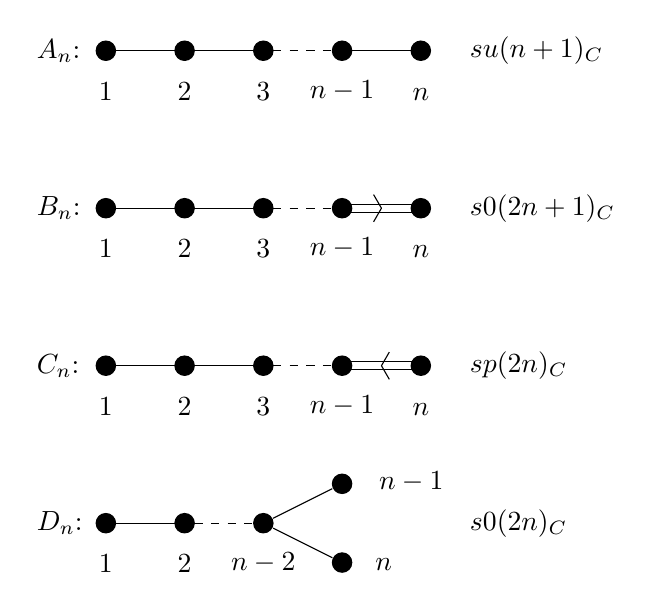
\begin{tikzpicture}

%-------------- An -------------------------------
  
\node [label={[yshift=-25pt]1}] (A1) at (-5,0) {};
\node [label={[yshift=-25pt]2}] (A2) at (-4,0) {};
\node [label={[yshift=-25pt]3}] (A3) at (-3,0) {};
\node [label={[yshift=-25pt]$n-1$}] (An1) at (-2,0) {};
\node [label={[yshift=-25pt]$n$}] (An) at (-1,0) {};

\draw [fill] (A1) circle (3.5pt)
(A2) circle (3.5pt)
(A3) circle (3.5pt)
(An1) circle (3.5pt)
(An) circle (3.5pt);

\draw  (A2) edge (A1);
\draw  (A2) edge (A3);
\draw [dashed] (A3) -- (An1);
\draw  (An1) edge (An);

\node [right] at (-6,0) {$A_n$:};

\node [right] at (-0.5,0) {$\rightsquigarrow \mathfrak{su}(n+1)_\mathbb{C}$};

%---------------- Bn -----------------------------
\node [label={[yshift=-25pt]1}] (B1) at (-5,-2) {};
\node [label={[yshift=-25pt]2}] (B2) at (-4,-2) {};
\node [label={[yshift=-25pt]3}] (B3) at (-3,-2) {};
\node [label={[yshift=-25pt]$n-1$}] (Bn1) at (-2,-2) {};
\node [label={[yshift=-25pt]$n$}] (Bn) at (-1,-2) {};


\draw [fill] (B1) circle (3.5pt)
(B2) circle (3.5pt)
(B3) circle (3.5pt)
(Bn1) circle (3.5pt)
(Bn) circle (3.5pt);

\draw  (B2) edge (B1);
\draw  (B2) edge (B3);
\draw [dashed] (B3) -- (Bn1);
\draw (-1,-1.95) -- (-2,-1.95);
\draw (-1,-2.05) -- (-2,-2.05);

% makes the arrow head
\draw
(-1.5,-2) --++(120:0.2)
(-1.5,-2) --++(-120:0.2);

\node [right] at (-6,-2) {$B_n$:};


\node [right] at (-0.5,-2) {$\rightsquigarrow \mathfrak{s0}(2n+1)_\mathbb{C}$};

%---------------- Cn ------------------------------

\node [label={[yshift=-25pt]1}] (C1) at (-5,-4) {};
\node [label={[yshift=-25pt]2}] (C2) at (-4,-4) {};
\node [label={[yshift=-25pt]3}] (C3) at (-3,-4) {};
\node [label={[yshift=-25pt]$n-1$}] (Cn1) at (-2,-4) {};
\node [label={[yshift=-25pt]$n$}] (Cn) at (-1,-4) {};
\draw (-1,-3.95) -- (-2,-3.95);
\draw (-1,-4.05) -- (-2,-4.05);

\draw [fill] (C1) circle (3.5pt)
(C2) circle (3.5pt)
(C3) circle (3.5pt)
(Cn1) circle (3.5pt)
(Cn) circle (3.5pt);

\draw  (C2) edge (C1);
\draw  (C2) edge (C3);
\draw [dashed] (C3) -- (Cn1);
\draw (-1,-1.95) -- (-2,-1.95);
\draw (-1,-2.05) -- (-2,-2.05);

% makes the arrow head
\draw
(-1.5,-4) --++(60:0.2)
(-1.5,-4) --++(-60:0.2);

\node [right] at (-6,-4) {$C_n$:};

\node [right] at (-0.5,-4) {$\rightsquigarrow \mathfrak{sp}(2n)_\mathbb{C}$};

%---------------- Dn ------------------------------

\node  [label={[yshift=-25pt]1}] (D1) at (-5,-6) {};
\node  [label={[yshift=-25pt]2}] (D2) at (-4,-6) {};
\node  [label={[yshift=-25pt]$n-2$}] (Dn2) at (-3,-6) {};
\node  [label={[xshift=25pt, yshift=-10pt]$n-1$}] (Dn1) at (-2,-5.5) {};
\node  [label={[xshift=15pt, yshift=-10pt]$n$}] (Dn) at (-2,-6.5) {};


\draw [fill] (D1) circle (3.5pt)
(D2) circle (3.5pt)
(Dn2) circle (3.5pt)
(Dn1) circle (3.5pt)
(Dn) circle (3.5pt);



\draw  (D1) edge (D2);
\draw [dashed] (D2) edge (Dn2);
\draw  (Dn2) edge (Dn1);
\draw  (Dn2) edge (Dn);

\node [right] at (-6,-6) {$D_n$:};

\node [right] at (-0.5,-6) {$\rightsquigarrow \mathfrak{s0}(2n)_\mathbb{C}$};

\end{tikzpicture}
\\
	where $n = \text{Rank}(\mathfrak{g})$, as well as the special cases
		\begin{center}
			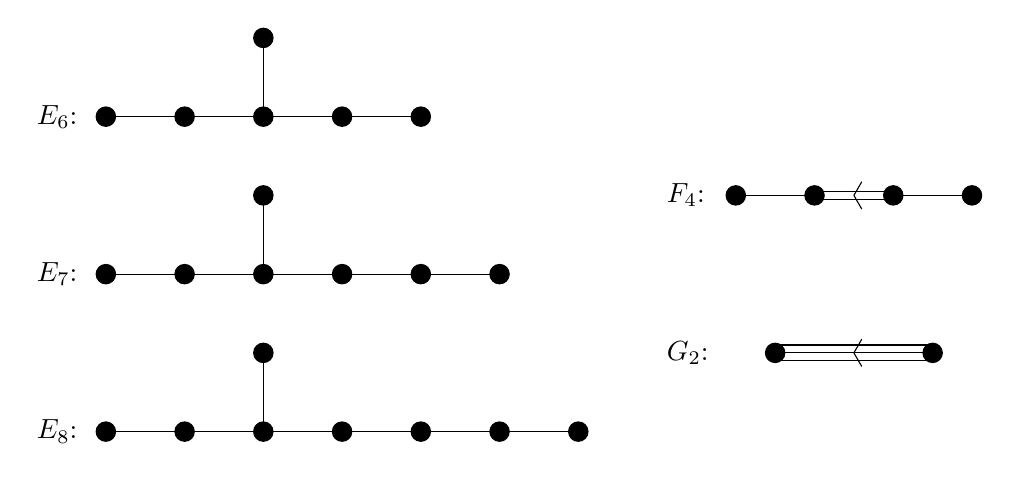
\begin{tikzpicture}
%-------------- E6 --------------------
\node (E61) at (-2,2) {};
\node (E62) at (-3,2) {};
\node (E63) at (-4,2) {};
\node (E64) at (-3,3) {};
\node (E65) at (-5,2) {};
\node (E66) at (-1,2) {};

\draw  (E65) edge (E63);
\draw  (E63) edge (E62);
\draw  (E62) edge (E64);
\draw  (E62) edge (E61);
\draw  (E61) edge (E66);

\draw [fill] 
(E61) circle (3.5pt)
(E62) circle (3.5pt)
(E63) circle (3.5pt)
(E64) circle (3.5pt)
(E65) circle (3.5pt)
(E66) circle (3.5pt)
;

\node [right] at (-6,2) {$E_6$:};
%--------------- E7 ----------------------

\node (E71) at (-2,0) {};
\node (E72) at (-3,0) {};
\node (E73) at (-4,0) {};
\node (E74) at (-3,1) {};
\node (E75) at (-5,0) {};
\node (E76) at (-1,0) {};
\node (E77) at (0,0) {};

\draw  (E75) edge (E73);
\draw  (E73) edge (E72);
\draw  (E72) edge (E74);
\draw  (E72) edge (E71);
\draw  (E71) edge (E76);
\draw  (E76) edge (E77);

\draw [fill] 
(E71) circle (3.5pt)
(E72) circle (3.5pt)
(E73) circle (3.5pt)
(E74) circle (3.5pt)
(E75) circle (3.5pt)
(E76) circle (3.5pt)
(E77) circle (3.5pt)
;

\node [right] at (-6,0) {$E_7$:};
%--------------- E8 ----------------------

\node (E81) at (-2,-2) {};
\node (E82) at (-3,-2) {};
\node (E83) at (-4,-2) {};
\node (E84) at (-3,-1) {};
\node (E85) at (-5,-2) {};
\node (E86) at (-1,-2) {};
\node (E87) at (0,-2) {};
\node (E88) at (1,-2) {};

\draw  (E85) edge (E83);
\draw  (E83) edge (E82);
\draw  (E82) edge (E84);
\draw  (E82) edge (E81);
\draw  (E81) edge (E86);
\draw  (E86) edge (E87);
\draw  (E87) edge (E88);

\draw [fill] 
(E81) circle (3.5pt)
(E82) circle (3.5pt)
(E83) circle (3.5pt)
(E84) circle (3.5pt)
(E85) circle (3.5pt)
(E86) circle (3.5pt)
(E87) circle (3.5pt)
(E88) circle (3.5pt)
;

\node [right] at (-6,-2) {$E_8$:};

%--------------- F4 ----------------------

\node [right] at (2,1) {$F_4$:};

\node (F1) at (3,1) {};
\node (F2) at (4,1) {};
\node (F3) at (5,1) {};
\node (F4) at (6,1) {};

\draw [fill]
(F1) circle (3.5pt)
(F2) circle (3.5pt)
(F3) circle (3.5pt)
(F4) circle (3.5pt)
;

\draw  (F1) edge (F2);
\draw  (F3) edge (F4);

\draw (4,1.05) -- (5,1.05);
\draw (4,0.95) -- (5,0.95);

\draw
(4.5,1) --++(60:0.2)
(4.5,1) --++(-60:0.2);
%--------------- G2 ----------------------


\node [right] at (2,-1) {$G_2$:};

\node (G1) at (3.5,-1) {};
\node (G2) at (5.5,-1) {};

\draw [fill]
(G1) circle (3.5pt)
(G2) circle (3.5pt)
;

\draw (3.5,-0.9) -- (5.5,-0.9);
\draw (3.5,-1) -- (5.5,-1);
\draw (3.5,-1.1) -- (5.5,-1.1);

\draw
(4.5,-1) --++(60:0.2)
(4.5,-1) --++(-60:0.2);

\end{tikzpicture}
		\end{center}
\end{theorem}
\begin{remark}\hfill
	\begin{itemize}
		\item $A_1 \simeq B_1 \simeq C_1 \simeq D_1$ ($\Rightarrow \mathfrak{su}(2)_\mathbb{C} \simeq \mathfrak{so}(3)_\mathbb{C} \simeq \mathfrak{sp}(2)_\mathbb{C}$),
		\item $B_2 \simeq C_2$ ($\Rightarrow \mathfrak{so}(5)_\mathbb{C} \simeq \mathfrak{sp}(4)_\mathbb{C}$),
		\item $D_2 \simeq A_1 \oplus A_1$ ($\Rightarrow \mathfrak{so}(4)_\mathbb{C} \simeq \mathfrak{su}(2)_\mathbb{C} \oplus \mathfrak{su}(2)_\mathbb{C}$),
		\item $D_3 \simeq A_3$ ($\Rightarrow \mathfrak{so}(6)_\mathbb{C} \simeq \mathfrak{su}(4)_\mathbb{C}$).
	\end{itemize}
\end{remark}

\section{Reconstructing the Lie Algebra}

\paragraph{} Given a Dynkin diagram/Cartan matrix, we immediately know about the simple roots, and also have $3 \cdot \text{Rank}(\mathfrak{g})$ generators for the Lie algebra from the Chevalley-Serre relations \eqref{eq:C-S1} and \eqref{eq:C-S2}. The challenge then is to construct the rest of the root system

\begin{theorem}
	To find the positive roots $\Phi_+$ from the simple roots $\Phi_s$ of a simple Lie algebra, it is sufficient to consider root strings of the form
		\begin{equation*}
			\delta + n \alpha_{(i)},
		\end{equation*}
	where $\delta \in \Phi_+$ and $\alpha_{(i)} \in \Phi_S$.
\end{theorem}

\paragraph{} Specifically we need the following facts:
	\begin{itemize}
		\item Positive roots can always be expressed as a sum of simple roots with \textit{positive} integer coefficients. Hence there can be no roots $ \alpha \in \Phi $ which have a mixture of positive and negative coefficients of the simple roots.
		\item For any two roots $ \alpha, \beta $, $ S_{\alpha,\beta} $ generates a finite dimensional irreducible representations of $ \mathfrak{sl}(2;\mathbb{C}) $ where
			\begin{equation}\label{key}
				R(H)e^\gamma = 2\frac{(\alpha,\gamma)}{(\alpha, \alpha)} e^\gamma,
				\qquad \forall \gamma \in S_{\alpha,\beta}.
			\end{equation} 
		Specifically, this allows us to invoke a convexity argument that if $ \gamma = \beta + m \alpha \in S_{\alpha,\beta} $, then $ \{ \beta + n \alpha : n \in {-|m|, -|m| + 1, \cdots, |m|} \} \subset  S_{\alpha\beta} $.
	\end{itemize}
Combining these results with the above theorem we see that the $ \min(S_{\alpha,\beta}) \geq 0 $
\todo[inline]{Reconstruction from $ G_2 $}

\begin{example}[Reconstructing $\mathfrak{su}(3)_\mathbb{C}$ from $A_2$]
	Reading off from the Dynkin diagram, we see that
		\begin{equation}
			A_2 = \begin{pmatrix}
				2 & -1 \\ -1 & 2
			\end{pmatrix}.
		\end{equation}
	Label the simple roots $\alpha$ and $\beta$. For both the $\alpha$ string through $\beta$ and vice versa, $n_+ = 1$, thus from either we obtain a single new root $\delta = (\alpha + \beta)$. Now, the result that $n_- = 0$ for simple root strings did \textit{not} require the `through' root to be simple, thus $n_- = 0$ for both the $\alpha$ string through $\delta$ and the $\beta$ string, and 
		\begin{align}\begin{split}\label{eq:simpleThroughPositive}
			\ell_{\alpha \delta} 
			&= 1 - 2\frac{(\alpha, \delta)}{(\alpha, \alpha)} \\
			&= 1 - \left( 2 \frac{(\alpha, \alpha)}{(\alpha, \alpha)} + 2 \frac{(\alpha, \beta)}{(\alpha, \alpha)}\right)\\
			&= 1 - \left( A^{11} + A^{21} \right) = 1 - (2 + (-1)) = 0.
		\end{split}\end{align}
	By symmetry, the same is true for $\ell_{\beta \delta}$. Thus, by the above theorem, we have exhausted all the possibilities for positive roots, and can write down our full root system
		\begin{equation}
			\Phi = \{ \alpha, \beta, \delta = (\alpha + \beta), -\alpha, -\beta, -\delta \}.
		\end{equation}
	From this root system, we can then write down the corresponding Cartan-Weyl basis for $\mathfrak{g}$
		\begin{equation}
			\mathfrak{g} = \text{Span}_\mathbb{C} \{ h^\alpha, h^\beta, e^{\pm \alpha}, e^{\pm \beta}, e^{\pm \delta} \},
		\end{equation}
	where the Lie brackets are given by \eqref{eq:sl2LikeBracket}
\end{example}

\begin{remark}
	From property (iv) of \autoref{prop:SimpleRootProps}, we know that any positive root can be expressed as $\delta = \sum_{i=1}^r m_i \alpha_{(i)}$, for some integers $m_i \geq 0$. Similarly to \eqref{eq:simpleThroughPositive}, we can deduce that
		\begin{equation}
			\ell_{\alpha_{(j)} \delta} = 1 - \sum_{i=1}^r A^{ij}m_i.
		\end{equation}
\end{remark}

\subsection{Representations of $\mathfrak{g}$}
\begin{definition}[Weight Space]
	Suppose that we have some representation of a Lie algebra $R: \mathfrak{g} \to GL(V)$ such that $R(H)$ is diagonalisable $\forall H \in \mathfrak{h}$. Then a \textbf{weight space} is some subspace $V_\lambda \subset V$, indexed by a functional $\lambda \in \mathfrak{h}^*$, known as a \textbf{weight}, such that $\forall v \in V_\lambda$
		\begin{equation}
			R(H)v = \lambda(H) v.
		\end{equation}
\end{definition}
\begin{remark}
	If $R$ is the adjoint rep of $\mathfrak{g}$, then the weights of the rep are just the roots of $\mathfrak{g}$.
\end{remark}
\begin{prop}[Some Facts About Weights of Representations] \hspace*{\fill}
	\begin{ronumerate}
		\item Let $S$ denote the set of weights of a representation, the representation space is then spanned by
			\begin{equation}\label{eq:CrudeWeightSpan}
				V = \bigoplus_{\lambda \in S_R} V_\lambda,
			\end{equation}
		\item For a weight $\lambda$ and root $\alpha$, if $\lambda + \alpha$ is also a weight, then
			\begin{equation}
				R(e^\alpha) : V_\lambda \to V_{\lambda + \alpha}.
			\end{equation}
		\item For a weight $\lambda$ and \textit{simple} root $\alpha_{(i)}$, $v \in V_\lambda$
			\begin{equation}
				R(h^\alpha)v = 2\frac{(\alpha_{(i)}, \lambda)}{(\alpha_{(i)}, \alpha_{(i)})} \in \mathbb{Z}
			\end{equation}
	\end{ronumerate}
\end{prop}
\begin{proof}\hfill
	\begin{ronumerate}
		\item This is simply a consequence of the assumption that all $R(H)$ are diagonalisable, as they share an eigenbasis which spans the vector space.
		\item Let $v \in V_\lambda$, assuming $R(e^\alpha)v \neq 0$, we have
			\begin{align}
				\begin{split}
					R(H) \left[ R(e^\alpha) v \right] 
					&= R(e^\alpha) R(H) v + R\left( \left[ H, e^\alpha \right] \right) v\\
					&= \lambda(H) \left[R(e^\alpha) v \right]  + \alpha(H) \left[R(e^\alpha) v \right] \\
					&= (\lambda + \alpha)(H) \left[R(e^\alpha) v \right].
				\end{split}
			\end{align}
		\item Recall \eqref{eq:rootInnerProdDef}, which tells us that $\lambda(H^\alpha) = (\alpha,\lambda)$, this works as $\kappa$ induces an isomorphism between $\mathfrak{h}$ and \textit{all of} $\mathfrak{h}^*$, not just roots. Then the rescaling of $H^\alpha$ \eqref{eq:HRescale} gives the desired equality. To prove that this is integral, consider the $\mathfrak{sl}(2)_\alpha$ subalgebra of $\mathfrak{g}$. Let $S_{\alpha, \lambda} \coloneqq \{ \lambda  + n \alpha \in S : n = \mathbb{Z} \} $, then 
			\begin{equation}
				V_\alpha \coloneqq \bigoplus_{\mu \in S_{\alpha, \lambda}} V_\mu
			\end{equation}
		is a representation space of $\mathfrak{sl}(2; \mathbb{C})$ with weights $\frac{2 (\alpha, \mu)}{(\alpha, \alpha)}$.\footnote{For completeness, the representation is $H \mapsto R(h^\alpha)$, $E^\pm \mapsto R(e^{\pm \alpha})$, note that the rescaled algebra was needed for the Lie algebra isomorphism to have the correct coefficients for the Lie brackets.} From our representation theory of $\mathfrak{sl}(2;\mathbb{C})$ we know that these weight must be integers.
	\end{ronumerate}
\end{proof}

\subsection{Root and Weight Lattices}

\begin{remark}
	There was a glaring omission in \eqref{eq:CrudeWeightSpan}, namely, \textit{what weights does a given representation admit}?
\end{remark}

\begin{definition}[Root/Co-root Lattice]
	Given a set of simple roots $\Phi_S$ for a root system $\Phi$, the \textbf{root lattice} is the superset of $\Phi$ defined by
		\begin{equation}
			\mathcal{L}[\mathfrak{g}] \coloneqq \text{Span}_\mathbb{Z} \Phi_S.
		\end{equation}
	If we define the \textbf{co-roots} associated to $\Phi_S$ as
		\begin{align}\label{eq:corootDef}
			\check{\alpha}_{(i)} \coloneqq \frac{2 \alpha_{(i)}}{(\alpha_{(i)}, \alpha_{(i)})},
		\end{align}
	then the \textbf{co-root lattice} is
		\begin{equation}
			\check{\mathcal{L}}(\mathfrak{g}) \coloneqq \text{Span}_\mathbb{Z} \{ \check{\alpha}_{(i)} \}_{i=1}^r.
		\end{equation}
\end{definition}

\begin{definition}[Dual Lattice \& Weight Lattice]
		Given a vector space $V$ with inner product $(\cdot,\cdot)$. The \textbf{dual} of a lattice $\mathcal{L}$ with respect to the inner product is defined by
			\begin{equation}
				\mathcal{L}^* \coloneqq \{ v \in V : (u,v) \in \mathbb{Z}, \forall u \in \mathcal{L} \}.
			\end{equation}
		The \textbf{weight lattice} $\mathcal{L}_W [\mathfrak{g}]$ is the dual of the co-root lattice, explicitly
			\begin{equation}\label{eq:weightLatticeExplicit}
				\mathcal{L}_W[\mathfrak{g}] = \left\{ \lambda \in \mathfrak{h}^* : \frac{2(\alpha_{(i)},\lambda)}{(\alpha_{(i)},\alpha_{(i)})} \in \mathbb{Z}, i = 1, \cdots, r \right\}
			\end{equation}
\end{definition}

\begin{definition}[Fundamental weights]
	A basis of the co-root lattice $\{\check{\alpha}_{(i)}\}$ induces a basis for the weight lattice $\{\omega_{(i)}\}$ satisfying
		\begin{equation}\label{eq:FundWeighDef}
			(\check{\alpha}_{(i)}, \omega_{(j)} ) = \delta_{ij}.
		\end{equation}
	These are then referred to as the \textbf{fundamental weights} of $\mathfrak{g}$
\end{definition}

\begin{definition}[Dynkin Labels]
	Given a basis of fundamental weights for $\mathcal{L}_W[\mathfrak{g}]$, the coordinates of $\lambda \in \mathcal{L}_W[\mathfrak{g}]$ form a tuple $(\lambda^i)$ known as the \textbf{Dynkin labels} of the weight $\lambda$.
\end{definition}

\begin{remark}
	As the simple roots form a basis of $\mathfrak{h}^*_\mathbb{R}$, we can express the fundamental weights as
		\begin{equation}
			\omega_{(i)} = \sum_{j=1}^r B_i^j \alpha_{(j)}.
		\end{equation}
	Substituting this and \eqref{eq:corootDef} into \eqref{eq:FundWeighDef} we see that
		\begin{equation} 
			\sum_{k=1}^r \frac{2 B^k_j}{(\alpha_{(i)}, \alpha_{(i)})} (\alpha_{(i)}, \alpha_{(k)}) = \sum_{k=1}^r B^k_j A_{ki} = \delta_{ij}.
		\end{equation}
	Thus $B$ is the inverse of $A$, i.e.
		\begin{equation}
			\alpha_{(i)} = \sum_{j=1}^r A_i^j \omega_{(j)}.
		\end{equation}
\end{remark}

\subsection{Highest Weight Representations}

\begin{prop}
	Every finite dimensional irreducible representation $R:\mathfrak{g} \to GL(V)$ has a \textbf{highest weight} $\Lambda \in \mathcal{L}_W[\mathfrak{g}]$ with respect to some choice of $\Phi_+$ such that, $\forall v \in V_{\Lambda}, \alpha \in \Phi_+$, $R(e^\alpha) v = 0$. Further more, all other weights of the representation are of the form
		\begin{equation}\label{eq:weightSpan}
			\lambda = \Lambda - \sum_{i=1}^r \mu^i \alpha_{(i)},
		\end{equation}
	for some $\mu^i \in \mathbb{Z}^+$. The highest weight characterises a representation uniquely up to isomorphism.
\end{prop}
\begin{proof}[Proof (partial)]
	The argument works similarly to that of the special case $\mathfrak{su}(2)_\mathbb{C}$. Let $\Lambda$ be any weight of $R$. If $R(e^\alpha): V_\Lambda \to \{ 0\} \forall \alpha \in \Phi_+$, then we are done. If not, then we can find some $\alpha \in \Phi_+$ such that $\Lambda + \alpha$ is a root. Relabel this to be our new $\Lambda$. We can repeat this process only finitely many times, as each weight space is linearly independent of the rest - by the same argument as for $\mathfrak{su}(2)_\mathbb{C}$ - and by hypothesis the rep space is finite dimensional. To prove \eqref{eq:weightSpan}, we rely on the fact that $V$ is irreducible. Recall that if $\Lambda - \alpha$ is a weight, then $R(e^{-\alpha}) : V_\Lambda \to V_{\Lambda - \alpha}$. By acting on $V_\Lambda$ by arbitrarily many step operators, we obtain a set of weights $\tilde{S}_R = \{ \Lambda - \sum_i \mu^i \alpha_{(i)} \in S_R : \mu^i \in \mathbb{Z} \}$. We need only use simple roots as $\Phi \subset \mathcal{L}[\mathfrak{g}]$. As this is an invariant subspace, and $R$ is irreducible, $U = V$, and $\tilde{S}_R = S_R$. Finally, that the integers $\mu^i$ must be positive follows from the definition of $\Lambda$, as if we have some $\mu^j < 0$, then $\Lambda + \mu^j \alpha_{(j)}$ is a weight, which contradicts the selection of $\Lambda$ to be the highest weight.
\todo{Clean up/ complete}
\end{proof}
\begin{remark}
	What is missing from this proof some sort of convexity argument, that $\lambda - n \alpha_{(i)} \in S_R \Rightarrow \lambda - m \alpha_{(i)} \forall 0 < m < n$.
\end{remark}

\begin{prop}
	If $\lambda = \sum_i \lambda^i \omega_{(i)} \in S_R$, then $\lambda - \sum_i m^i \alpha_{(i)} \in S_R \forall m^i \in \{0, 1, \cdots, \lambda^i \}$. In words, the Dynkin labels of a weight $\lambda$ tell us how many times the corresponding \textit{root} can be subtracted from that weight. Thus, if a weight has no positive roots, this result cannot be applied.
\end{prop}

\begin{example}[Representation Theory of $A_2$]
	As this is a rank $2$ Lie algebra, each weight has 2 Dynkin labels. Let the highest weight of a rep $R$ be $\Lambda \rightsquigarrow (\Lambda_1, \Lambda_2)$. It helps to note that the Dynkin labels of the simple roots are $\alpha_{(1)} \rightsquigarrow ( 2, -1), \alpha_{(2)} \rightsquigarrow (-1, 2)$. Thus, $\lambda = \Lambda - \sum_i \mu^i \alpha_{(i)}$ has Dynkin labels
		\begin{equation}
			(\lambda_1, \lambda_2) = (\Lambda_1 - 2\mu^1 + \mu^2, \Lambda_2 +\mu^1 -2\mu^2).
		\end{equation}
	The complete set of weights is then obtained through an application of the above proposition. Say we choose $\Lambda = (2,1)$, then we immediately have two `strings' of weights, of length $2$ and $1$ respectively. By considering all the strings possible through these new weights, we can continue to obtain the full set of weights:
			\begin{center}
				\input{A2RepPretty}
			\end{center}
	\textit{Note: if you ever need to do this in an exam, it is sufficient to draw the lattice orthogonally, e.g. left for $\alpha_{(2)}$, down for $\alpha_{(1)}$. The result should be something like:}
			\begin{center}
				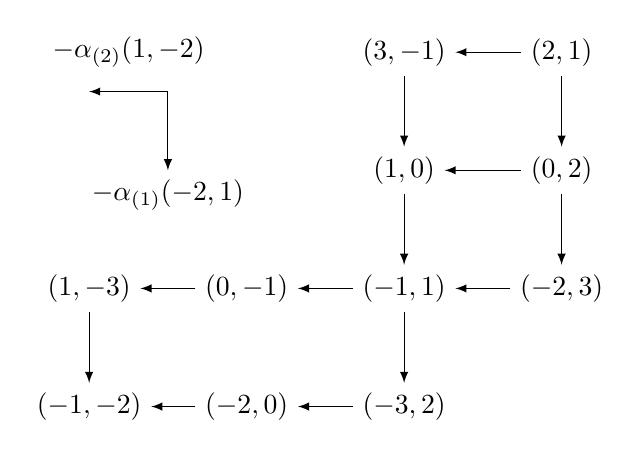
\begin{tikzpicture}

\node (v1) at (-4,-4.5) {$(2,1)$};
\node (v2) at (-4,-6) {$(0,2)$};
\node (v3) at (-4,-7.5) {$(-2,3)$};
\node (v4) at (-6,-4.5) {$(3,-1)$};
\draw [-latex] (v1) edge (v2);
\draw [-latex] (v2) edge (v3);
\draw [-latex] (v1) edge (v4);
\node (v5) at (-6,-6) {$(1,0)$};
\node (v6) at (-6,-7.5) {$(-1,1)$};
\node (v7) at (-6,-9) {$(-3,2)$};
\draw [-latex] (v4) edge (v5);
\draw [-latex] (v5) edge (v6);
\draw [-latex] (v6) edge (v7);
\draw [-latex] (v2) edge (v5);
\node (v8) at (-8,-7.5) {$(0,-1)$};
\node (v9) at (-10,-7.5) {$(1,-3)$};
\node (v10) at (-8,-9) {$(-2,0)$};
\node (v11) at (-10,-9) {$(-1,-2)$};
\draw [-latex] (v6) edge (v8);
\draw [-latex] (v8) edge (v9);
\draw [-latex] (v7) edge (v10);
\draw [-latex] (v10) edge (v11);
\draw [-latex] (v3) edge (v6);
\draw [-latex] (v9) edge (v11);


\draw [-latex] (-9,-5) -- (-9,-6);
\draw [-latex] (-9,-5) -- (-10,-5);
\node [below] at (-9,-6) {$ -\alpha_{(1)} \rightsquigarrow (-2,1)$};
\node at (-9.5,-4.5) {$-\alpha_{(2)} \rightsquigarrow (1,-2)$};

\end{tikzpicture}
			\end{center}
\end{example}

\section{Symmetries in Quantum Mechanics}

\begin{remark}
	Traditionally, in quantum mechanics, the Hilbert space of quantum states is decomposed into a direct sum of eigenspaces of the Hamiltonian
		\begin{equation}
			\mathcal{H} = \bigoplus_{n \geq 0} \mathcal{H}_n,
		\end{equation}
	where $|n\rangle \in \mathcal{H}_n \Rightarrow \hat{H}|n\rangle = E_n |n\rangle.$
\end{remark}

\begin{definition}[Symmetry Transformation]
	A \textbf{symmetry transformation} of a quantum system is an automorphism\footnote{Here we tacitly define an isomorphism between Hilbert spaces to be a map which preserves addition (i.e. is linear) and the inner product. Thus an \textit{auto}morphism is a unitary operator.} $\hat{U}$ on its Hilbert space $\mathcal{H}$ such that $\hat{U}\hat{H}\hat{U}^\dagger = \hat{H}$.
\end{definition}

\begin{definition}[Conserved Quantity]
	A \textbf{conserved quantity} is an observable $\hat{I} = \hat{I}^\dagger$ such that $[\hat{I},\hat{H}] = 0$.
\end{definition}
\begin{remark}
	If $\hat{I}$ commutes with $\hat{H}$, then so too does $e^{\alpha \hat{I}} \forall \alpha \in \mathbb{C}$. Further, if $\hat{I}$ is Hermitian, then $e^{i s \hat{I}}$ is unitary $\forall s \in \mathbb{R}$. Thus, if $\hat{I}$ is a conserved quantity, then it generates a family of symmetry transformations $e^{is\hat{I}}$. This is essentially a quantum Noether's theorem.
	
	Given a maximal set of linearly independent conserved quantities $\{\hat{I}^a\}_{a=1}^d$, then $\mathfrak{g} \coloneqq \text{Span}_\mathbb{R}\{\hat{I}^a\}_{a=1}^d$ forms a real Lie algebra, where the Lie bracket is given by commutation of the observables. The group $G$ formed by exponentiating $\mathfrak{g}$ leaves each $\mathcal{H}_n$ invariant, due to all of the operators commuting with $\hat{H}$. \textit{For reasons I cannot justify}, for each $n$, we can construct a representation of $R: \mathfrak{g} \to GL\left(\mathcal{H}_n\right)$ such that $R(x)$ is skew-Hermitian $\forall x \in \mathfrak{g}$. \textbf{It may have something to do with the fact that the exponential map gives unitary operators.}
\end{remark}
\todo[inline]{Finish}

\begin{appendix}
	
\section{Complex Vector Spaces}
Results to prove
\begin{itemize}
	\item 	Define compatibility of Euclidean and inner product
	\item	Orthogonal vs unitary operators
	\item	Acting on operators, $ \star \circ \dagger \circ T = \text{Id} $
	\item	Operator representatives of vectors/duals, relation to trace
\end{itemize}

\end{appendix}

\end{document}